\documentclass[12pt, a4paper]{report}

\usepackage{fontspec}
\setmainfont{texgyretermes}[
  Extension      = .otf,
  UprightFont    = *-regular,
  BoldFont       = *-bold,
  ItalicFont     = *-italic,
  BoldItalicFont = *-bolditalic
]
\setsansfont{texgyreheros}[
  Extension      = .otf,
  UprightFont    = *-regular,
  BoldFont       = *-bold,
  ItalicFont     = *-italic,
  BoldItalicFont = *-bolditalic,
  Scale          = 0.95
]
\setmonofont{texgyrecursor}[
  Extension      = .otf,
  UprightFont    = *-regular,
  BoldFont       = *-bold,
  ItalicFont     = *-italic,
  BoldItalicFont = *-bolditalic,
  Scale          = 0.88
]
\usepackage{polyglossia}
\setmainlanguage{vietnamese}
\setotherlanguage{english}

\usepackage{geometry}
\geometry{a4paper, top=2.5cm, bottom=2.5cm, left=3cm, right=2cm, headheight=15pt}
\usepackage{setspace}
\onehalfspacing
\usepackage{indentfirst}
\usepackage{fancyhdr}
\pagestyle{fancy}
\fancyhf{}
\fancyhead[L]{\small Phân tích \& Thiết kế thuật toán - Bài tập lớn}
\fancyhead[R]{\small\thepage}
\renewcommand{\headrulewidth}{0.4pt}

\usepackage{amsmath, amssymb, amsthm}
\usepackage{mathtools}

\usepackage{booktabs}
\usepackage{array}
\usepackage{multirow}
\usepackage{tabularx}
\usepackage{longtable}
\newcolumntype{L}{>{\raggedright\arraybackslash}X}
\newcolumntype{G}{>{\centering\arraybackslash}p{0.55cm}}
\usepackage{graphicx}
\usepackage{float}
\usepackage{needspace}
\usepackage{caption}

\usepackage{enumitem}
\usepackage{pifont}
\newcommand{\vong}[1]{\ding{\numexpr171+#1\relax}}

\usepackage{fancyvrb}
\usepackage{listings, xcolor}
\definecolor{codebg}{gray}{0.96}
\lstset{
  backgroundcolor = \color{codebg},
  basicstyle      = \ttfamily\small,
  keywordstyle    = \color{blue!70!black}\bfseries,
  commentstyle    = \color{green!45!black}\itshape,
  stringstyle     = \color{orange!80!black},
  numbers         = left,
  numberstyle     = \tiny\color{gray},
  numbersep       = 8pt,
  breaklines      = true,
  frame           = single,
  framesep        = 5pt,
  xleftmargin     = 18pt,
  showstringspaces= false,
  captionpos      = b,
  literate        = {->}{{$\rightarrow$}}1 {<=}{{$\leq$}}1 {>=}{{$\geq$}}1
}

\usepackage[most]{tcolorbox}
\newtcolorbox{promptbox}[1]{
  colback=gray!4, colframe=gray!55!black, boxrule=0.5pt,
  title={Prompt · #1}, fonttitle=\small\bfseries, fontupper=\small,
  sharp corners=downhill, breakable
}
\newtcolorbox{ghichu}[1][Lưu ý]{
  colback=yellow!8, colframe=orange!70!black, boxrule=0.6pt,
  title=#1, fonttitle=\bfseries
}

\usepackage{hyperref}
\hypersetup{
  colorlinks = true, linkcolor = blue!60!black,
  urlcolor   = cyan!70!black, pdfstartview = FitH
}

\newcommand{\T}[1]{T\!\left(#1\right)}
\newcommand{\Oh}[1]{\mathcal{O}\!\left(#1\right)}
\newcommand{\Om}[1]{\Omega\!\left(#1\right)}
\newcommand{\Th}[1]{\Theta\!\left(#1\right)}
\newcommand{\lgn}{\log_2 n}
\DeclarePairedDelimiter{\floor}{\lfloor}{\rfloor}
\DeclarePairedDelimiter{\ceil}{\lceil}{\rceil}


\newcommand{\hoten}{Lã Xuân Hồng}
\newcommand{\mssv}{25410056}
\newcommand{\lophoc}{CS112.F31.LT.TTNT}
\newcommand{\giangvien}{Huỳnh Thị Thanh Thương}
\newcommand{\tenbaitap}{Bài tập lớn: Minh họa thuật toán quay lui qua bài toán Sudoku}

\begin{document}

\begin{titlepage}
  \centering
  {\large\bfseries ĐẠI HỌC QUỐC GIA TP. HỒ CHÍ MINH \\
   TRƯỜNG ĐẠI HỌC CÔNG NGHỆ THÔNG TIN \\
   KHOA KHOA HỌC MÁY TÍNH \par}

  \vspace{2.5cm}
  \rule{\linewidth}{0.5pt}\\[0.5cm]
  {\Huge\bfseries PHÂN TÍCH \& THIẾT KẾ \\[0.3cm] THUẬT TOÁN \par}
  \vspace{0.4cm}
  {\Large \tenbaitap \par}
  \rule{\linewidth}{0.5pt}\\[2cm]

  \begin{tabular}{@{}ll@{}}
    \textbf{Sinh viên thực hiện} & : \hoten \\[4pt]
    \textbf{MSSV}                & : \mssv \\[4pt]
    \textbf{Lớp}                 & : \lophoc \\[4pt]
    \textbf{Giảng viên hướng dẫn}& : \giangvien \\[4pt]
    \textbf{Ngày nộp bài}        & : \today \\
  \end{tabular}

  \vfill
  {\large TP. Hồ Chí Minh, \today \par}
\end{titlepage}

\tableofcontents

\chapter{Giới thiệu bài toán}

\section{Lý do chọn bài toán}

\section{Nguồn gốc của Sudoku}

\section{Ứng dụng thực tế}

\chapter{Mô tả bài toán}

Sudoku là trò chơi điền số trên lưới \(9 \times 9\). Lưới chia thành 9 khối \(3 \times 3\) bằng các đường kẻ đậm. Một lưới Sudoku hợp lệ khi mỗi hàng, mỗi cột và mỗi khối đều chứa đủ 9 số từ 1 đến 9, mỗi số đúng một lần.

Cho một lưới trong đó một số ô đã điền sẵn, các ô còn lại để trống. Hãy điền số vào các ô trống để được một lưới Sudoku hợp lệ, giữ nguyên các số đã cho.

\subsection*{Input}

Gồm 9 dòng, mỗi dòng 9 ký tự cách nhau bởi dấu cách. Mỗi ký tự là một số từ 1 đến 9 (ô đã điền) hoặc chữ \texttt{X} (ô trống). Số ô trống từ 0 đến 81.

\subsection*{Output}

\begin{itemize}
  \item Nếu điền được: 9 dòng, mỗi dòng 9 số cách nhau bởi dấu cách, là lưới đã điền kín và hợp lệ. Nếu có nhiều cách điền, xuất cách đầu tiên tìm được khi xét ô trống theo thứ tự hàng rồi cột và thử số từ nhỏ đến lớn.
  \item Nếu đề có hai ô cùng số trong cùng một hàng, cột hoặc khối: thông báo đề không hợp lệ, kèm số trùng và vị trí.
  \item Nếu không có cách điền nào: thông báo đề không có lời giải.
\end{itemize}

\subsection*{Ví dụ}

\begin{center}
  \begin{minipage}[t]{0.44\linewidth}
    \textbf{Input}
    \begin{Verbatim}[fontsize=\small, frame=single]
5 3 4 6 7 X 9 X X
6 7 X X 9 5 3 4 8
X 9 8 3 4 X 5 6 7
8 X 9 7 6 X X 2 3
4 X 6 X 5 3 7 9 1
7 1 3 9 X 4 8 5 6
9 6 1 5 3 7 2 X 4
2 8 7 4 1 9 6 3 5
X 4 5 X 8 6 1 7 9
\end{Verbatim}

  \end{minipage}
  \hfill
  \begin{minipage}[t]{0.44\linewidth}
    \textbf{Output}
    \begin{Verbatim}[fontsize=\small, frame=single]
5 3 4 6 7 8 9 1 2
6 7 2 1 9 5 3 4 8
1 9 8 3 4 2 5 6 7
8 5 9 7 6 1 4 2 3
4 2 6 8 5 3 7 9 1
7 1 3 9 2 4 8 5 6
9 6 1 5 3 7 2 8 4
2 8 7 4 1 9 6 3 5
3 4 5 2 8 6 1 7 9
\end{Verbatim}

  \end{minipage}
\end{center}

\subsection*{Yêu cầu}

Giải bằng kỹ thuật quay lui theo mô hình 1. Chương trình phải cho người dùng nhập đề, theo dõi từng bước thuật toán thực hiện, và xem kết quả.

\chapter{Mô hình bài toán}

\section{Input}

\section{Output}

\section{Điều kiện và ràng buộc}

\section{Ví dụ Input và Output}

\chapter{Thiết kế cấu trúc dữ liệu và thuật toán}

\section{Phân tích đặc trưng và ý tưởng giải}

\section{Cấu trúc dữ liệu}

\section{Thuật toán quay lui theo mô hình 1}

\section{Phân tích độ phức tạp}

\section{Các biến thể đã phát triển thêm}

\section{Cấu trúc dữ liệu của phần minh họa từng bước}

\chapter{Ví dụ minh họa các bước thực hiện}

Ví dụ của chương này là đề số 13, tên ``Ngắn, có quay lui'' trong danh sách đề mẫu của website. Đề có 16 ô trống và đúng một lời giải. Thuật toán cần 79 lần thử, ghi nhận 19 lần và trả lại 3 lần: một lần ở giai đoạn 1, hai lần ở giai đoạn 2. Hai lần ở giai đoạn 2 hợp thành một chuỗi lùi dây chuyền qua hai ô. Toàn bộ 83 bước nằm trong Bảng \ref{tab:illustration-steps} ở cuối chương.

\section{Chọn đề và cách đọc bảng}

Chương này cần một đề đủ ngắn để in trọn từng bước, mà vẫn có quay lui thật. Đề Arto Inkala cần 445.778 lần thử, quá dài. Đề ``Dễ'' chỉ cần 27 lần thử nhưng không quay lui lần nào. Claude viết script \texttt{checks/find\_illustration\_puzzle.py}: xóa ngẫu nhiên 10 đến 16 ô từ một lưới đầy, rồi giữ lại các đề thỏa đúng một lời giải, 50 đến 90 lần thử, 1 đến 3 lần quay lui, có đủ ba kiểu bị loại vì hàng, cột và khối. Trong 12 đề tìm được, Claude chọn đề này vì cả ba lần quay lui nằm gọn trong 35 lần thử đầu, ngay trên hàng 1.

\begin{figure}[H]
  \centering
  \begin{minipage}[t]{0.46\linewidth}
    \centering
    \begingroup\setlength{\tabcolsep}{0pt}\renewcommand{\arraystretch}{1.35}
\begin{tabular}{!{\vrule width 1.2pt}G|G|G!{\vrule width 1.2pt}G|G|G!{\vrule width 1.2pt}G|G|G!{\vrule width 1.2pt}}
\noalign{\hrule height 1.2pt}
\textbf{5} & \textbf{3} & \textbf{4} & \textbf{6} & \textbf{7} &  & \textbf{9} &  &  \\ \hline
\textbf{6} & \textbf{7} &  &  & \textbf{9} & \textbf{5} & \textbf{3} & \textbf{4} & \textbf{8} \\ \hline
 & \textbf{9} & \textbf{8} & \textbf{3} & \textbf{4} &  & \textbf{5} & \textbf{6} & \textbf{7} \\ \noalign{\hrule height 1.2pt}
\textbf{8} &  & \textbf{9} & \textbf{7} & \textbf{6} &  &  & \textbf{2} & \textbf{3} \\ \hline
\textbf{4} &  & \textbf{6} &  & \textbf{5} & \textbf{3} & \textbf{7} & \textbf{9} & \textbf{1} \\ \hline
\textbf{7} & \textbf{1} & \textbf{3} & \textbf{9} &  & \textbf{4} & \textbf{8} & \textbf{5} & \textbf{6} \\ \noalign{\hrule height 1.2pt}
\textbf{9} & \textbf{6} & \textbf{1} & \textbf{5} & \textbf{3} & \textbf{7} & \textbf{2} &  & \textbf{4} \\ \hline
\textbf{2} & \textbf{8} & \textbf{7} & \textbf{4} & \textbf{1} & \textbf{9} & \textbf{6} & \textbf{3} & \textbf{5} \\ \hline
 & \textbf{4} & \textbf{5} &  & \textbf{8} & \textbf{6} & \textbf{1} & \textbf{7} & \textbf{9} \\ \noalign{\hrule height 1.2pt}
\end{tabular}\endgroup

    \par\smallskip\small (a) Đề: 16 ô trống
  \end{minipage}
  \hfill
  \begin{minipage}[t]{0.46\linewidth}
    \centering
    \begingroup\setlength{\tabcolsep}{0pt}\renewcommand{\arraystretch}{1.35}
\begin{tabular}{!{\vrule width 1.2pt}G|G|G!{\vrule width 1.2pt}G|G|G!{\vrule width 1.2pt}G|G|G!{\vrule width 1.2pt}}
\noalign{\hrule height 1.2pt}
\textbf{5} & \textbf{3} & \textbf{4} & \textbf{6} & \textbf{7} & \textcolor{blue!65!black}{8} & \textbf{9} & \textcolor{blue!65!black}{1} & \textcolor{blue!65!black}{2} \\ \hline
\textbf{6} & \textbf{7} & \textcolor{blue!65!black}{2} & \textcolor{blue!65!black}{1} & \textbf{9} & \textbf{5} & \textbf{3} & \textbf{4} & \textbf{8} \\ \hline
\textcolor{blue!65!black}{1} & \textbf{9} & \textbf{8} & \textbf{3} & \textbf{4} & \textcolor{blue!65!black}{2} & \textbf{5} & \textbf{6} & \textbf{7} \\ \noalign{\hrule height 1.2pt}
\textbf{8} & \textcolor{blue!65!black}{5} & \textbf{9} & \textbf{7} & \textbf{6} & \textcolor{blue!65!black}{1} & \textcolor{blue!65!black}{4} & \textbf{2} & \textbf{3} \\ \hline
\textbf{4} & \textcolor{blue!65!black}{2} & \textbf{6} & \textcolor{blue!65!black}{8} & \textbf{5} & \textbf{3} & \textbf{7} & \textbf{9} & \textbf{1} \\ \hline
\textbf{7} & \textbf{1} & \textbf{3} & \textbf{9} & \textcolor{blue!65!black}{2} & \textbf{4} & \textbf{8} & \textbf{5} & \textbf{6} \\ \noalign{\hrule height 1.2pt}
\textbf{9} & \textbf{6} & \textbf{1} & \textbf{5} & \textbf{3} & \textbf{7} & \textbf{2} & \textcolor{blue!65!black}{8} & \textbf{4} \\ \hline
\textbf{2} & \textbf{8} & \textbf{7} & \textbf{4} & \textbf{1} & \textbf{9} & \textbf{6} & \textbf{3} & \textbf{5} \\ \hline
\textcolor{blue!65!black}{3} & \textbf{4} & \textbf{5} & \textcolor{blue!65!black}{2} & \textbf{8} & \textbf{6} & \textbf{1} & \textbf{7} & \textbf{9} \\ \noalign{\hrule height 1.2pt}
\end{tabular}\endgroup

    \par\smallskip\small (b) Lời giải: số in xanh là số thuật toán điền
  \end{minipage}
  \caption{Đề số 13 và lời giải}
  \label{fig:illustration-grids}
\end{figure}

Bảng \ref{tab:illustration-cells} đánh số 16 ô trống theo thứ tự hàng rồi cột. \(S_i\) là số điền vào ô trống thứ \(i\).

\begin{table}[H]
  \centering
  \caption{Vị trí của 16 ô trống}
  \label{tab:illustration-cells}
  \small
  \begin{tabular}{@{}l*{8}{c}@{}}
    \toprule
    \(i\) & 1 & 2 & 3 & 4 & 5 & 6 & 7 & 8 \\
    Ô & (1, 6) & (1, 8) & (1, 9) & (2, 3) & (2, 4) & (3, 1) & (3, 6) & (4, 2) \\
    \midrule
    \(i\) & 9 & 10 & 11 & 12 & 13 & 14 & 15 & 16 \\
    Ô & (4, 6) & (4, 7) & (5, 2) & (5, 4) & (6, 5) & (7, 8) & (9, 1) & (9, 4) \\
    \bottomrule
  \end{tabular}
\end{table}

Trạng thái dữ liệu gồm lưới \texttt{grid}, vectơ \(S\) và ba mảng đánh dấu \texttt{rowUsed}, \texttt{columnUsed}, \texttt{boxUsed} (Chương 4). Mỗi dòng của Bảng \ref{tab:illustration-steps} là một bước thuật toán:

\begin{itemize}
  \item \textbf{Bấm}: số lần bấm nút Từng bước trên trang Giải Sudoku để tới đúng trạng thái đó. Mỗi lần bấm, trang đi một sự kiện, kể cả các sự kiện không có dòng riêng trong bảng như ``ghi nhận'' và ``sang ô kế''. Vì vậy sau mỗi dòng Chấp nhận, cột Bấm tăng 3 (chấp nhận, ghi nhận, sang ô kế). Sau dòng Bị loại hay Trả lại, cột Bấm tăng 1. Ở ô cuối cùng, lần bấm 118 là chấp nhận, lần bấm 119 là ghi nhận, lần bấm 120 là xuất lời giải.
  \item \textbf{Lần thử}, \(i\), \textbf{Ô}, \(j\): bộ đếm lần thử, ô trống thứ mấy, nằm ở đâu, và số đang thử. Dòng Trả lại không tính là một lần thử, nên giữ nguyên bộ đếm của dòng trước, và \(j\) ở dòng đó là số vừa bị xóa.
  \item \textbf{Thao tác} và \textbf{Lý do}: ``Chấp nhận'' là số \(j\) chấp nhận được, thuật toán ghi nhận rồi sang ô trống kế tiếp. ``Bị loại'' kèm hàng, cột hoặc khối bị trùng và ô đang giữ số đó. Số trùng ở nhiều chỗ thì bảng ghi chỗ đầu tiên theo thứ tự hàng, cột, khối, đúng thứ tự thuật toán kiểm tra. ``Trả lại'' là trả lại trạng thái cũ vì ô phía sau đã hết số để thử. ``Có lời giải'' là dòng cuối, không thử thêm số nào, nên bộ đếm lần thử vẫn là 79.
  \item \textbf{\(S\) sau bước}: vectơ \(S_1 \ldots S_{16}\) sau khi bước đó xong, dấu chấm là thành phần chưa có giá trị.
\end{itemize}

Muốn kiểm lại trên website, mở trang Giải Sudoku, chọn ``Đề 13 - Ngắn, có quay lui'' ở ô Đề mẫu, rồi bấm Từng bước. Nút ``Tới lần quay lui kế'' đưa thẳng tới dòng Trả lại kế tiếp, nút ``Lùi một bước'' đi ngược lại. Bộ đếm trên trang cộng dồn từ đầu: 3 ghi nhận nghĩa là thuật toán đã ghi nhận 3 lần, không phải lưới đang có 3 số do thuật toán điền.

\section{Diễn biến}

Hàng 1 đã có các số 5, 3, 4, 6, 7, 9, nên ba ô trống \((1, 6)\), \((1, 8)\), \((1, 9)\) phải nhận đúng ba số 1, 2, 8. Số 8 đã nằm ở ô \((2, 9)\), cùng cột 9 với ô \((1, 9)\) và cùng khối 3 với cả hai ô \((1, 8)\), \((1, 9)\). Vậy chỉ ô \((1, 6)\) nhận được số 8. Người giải bằng tay thấy ngay điều này. Thuật toán thì thử từ nhỏ lên lớn, nên phải đi vào ngõ cụt hai lần mới tới số 8.

\subsection*{Giai đoạn 1: lần thử 1 đến 10, quay lui một ô}

Ở lần thử 1, thuật toán thử số 1 ở ô \((1, 6)\). Hàng 1, cột 6 và khối 2 đều chưa có số 1, nên số 1 chấp nhận được. Thuật toán ghi nhận: \(S_1 = 1\), \texttt{grid[1][6] = 1}, bật \texttt{rowUsed[1][1]}, \texttt{columnUsed[6][1]}, \texttt{boxUsed[2][1]}. Rồi sang ô trống thứ 2.

Ở ô \((1, 8)\), cả 9 số đều trùng. Số 1 trùng ngay với số vừa điền ở ô \((1, 6)\). Số 2 trùng cột 8, số 8 trùng khối 3, các số còn lại trùng hàng 1. Ô \((1, 8)\) hết số, nên sau lần thử 10, ở lần bấm 13, thuật toán trả lại trạng thái cũ của ô \((1, 6)\): xóa số 1 khỏi lưới, tắt ba cờ vừa bật, \(S_1\) trở về trống (Hình \ref{fig:press-13}).

\begin{figure}[H]
  \centering
  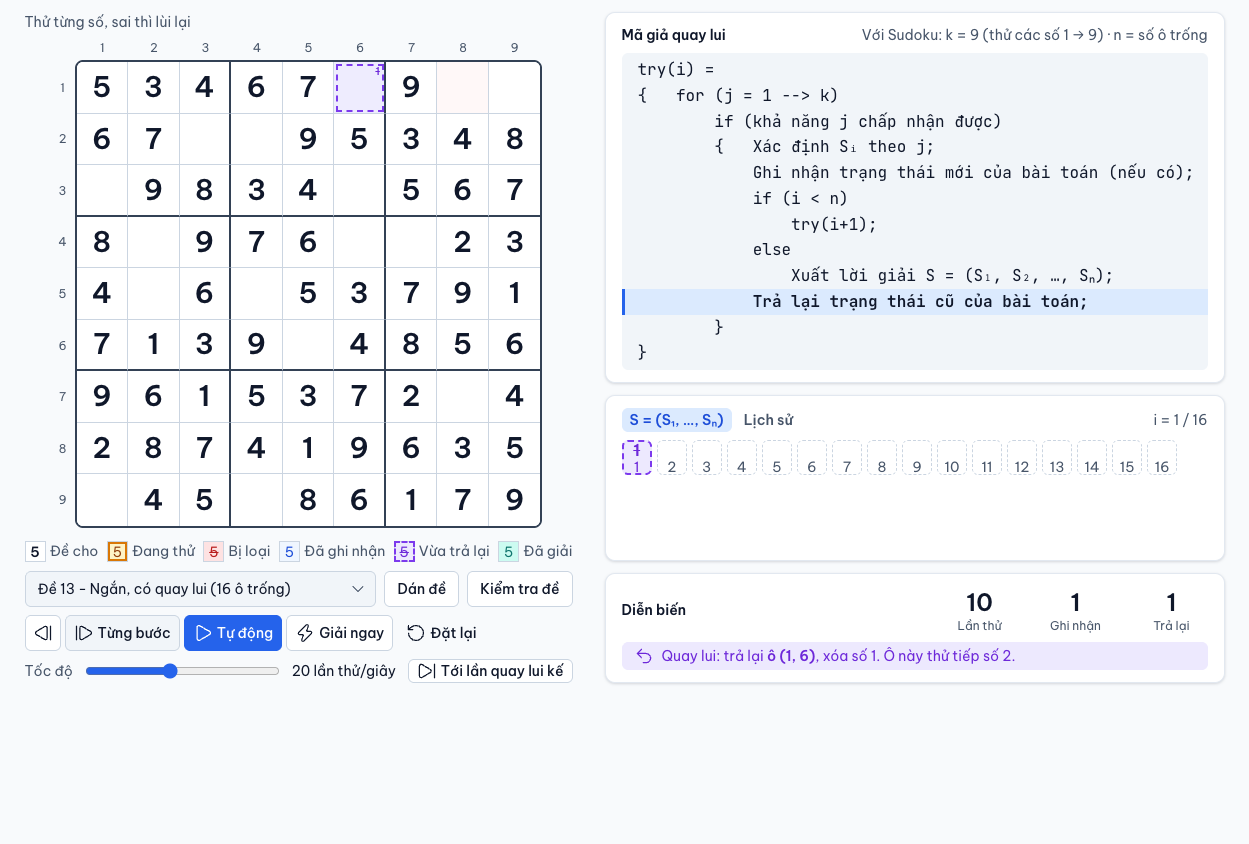
\includegraphics[width=0.95\linewidth]{figures/illustration-press-13.png}
  \caption{Lần bấm 13: thuật toán vừa trả lại ô (1, 6), xóa số 1. Bộ đếm: 10 lần thử, 1 ghi nhận, 1 trả lại}
  \label{fig:press-13}
\end{figure}

\subsection*{Giai đoạn 2: lần thử 11 đến 29, quay lui dây chuyền}

Thuật toán thử tiếp số 2 ở ô \((1, 6)\), và số 2 chấp nhận được (lần thử 11). Lần này ô \((1, 8)\) nhận được số 1, vì số 1 không còn ở hàng 1 nữa (lần thử 12). Ở ô trống thứ 3, ô \((1, 9)\), cả 9 số đều trùng: số 1 trùng với ô \((1, 8)\) vừa điền, số 2 trùng với ô \((1, 6)\), số 8 trùng cột 9, các số còn lại trùng hàng 1. Sau lần thử 21, ở lần bấm 29, thuật toán trả lại ô \((1, 8)\), xóa số 1 (Hình \ref{fig:press-29}).

\begin{figure}[H]
  \centering
  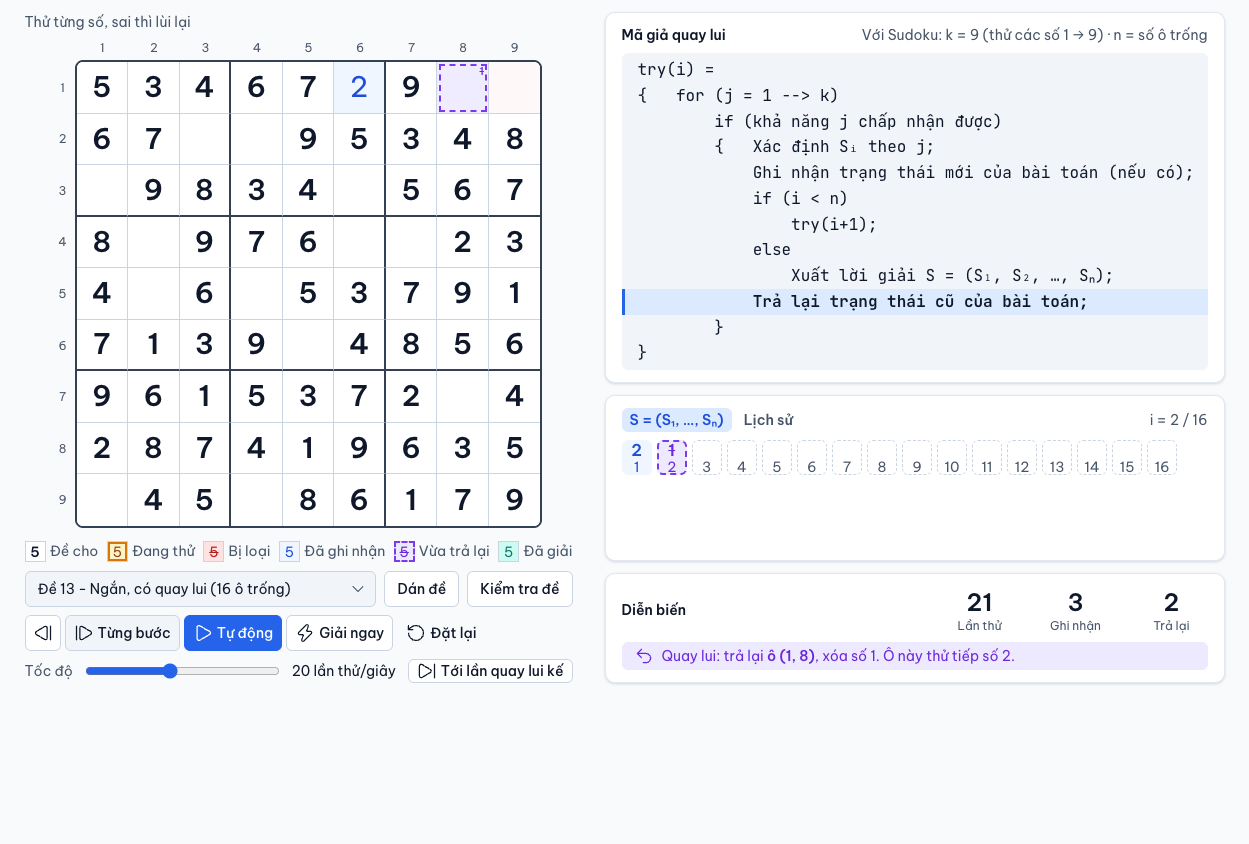
\includegraphics[width=0.95\linewidth]{figures/illustration-press-29.png}
  \caption{Lần bấm 29: thuật toán vừa trả lại ô (1, 8), xóa số 1. Bộ đếm: 21 lần thử, 3 ghi nhận, 2 trả lại}
  \label{fig:press-29}
\end{figure}

Ô \((1, 8)\) chưa hết số, nên thuật toán thử tiếp từ số 2. Số 2 trùng ô \((1, 6)\), số 8 trùng khối 3, các số còn lại trùng hàng 1. Ô \((1, 8)\) hết số lần thứ hai, nên sau lần thử 29, ở lần bấm 38, thuật toán lùi tiếp thêm một ô: trả lại ô \((1, 6)\), xóa số 2 (Hình \ref{fig:press-38}). Hình này gần giống Hình \ref{fig:press-13}. Chỗ khác là số bị gạch trong ô \(S_1\), nay là số 2, và bộ đếm. Đây là quay lui dây chuyền: ô \((1, 9)\) hết số làm ô \((1, 8)\) phải đổi số, và ô \((1, 8)\) hết số làm ô \((1, 6)\) phải đổi số.

\begin{figure}[H]
  \centering
  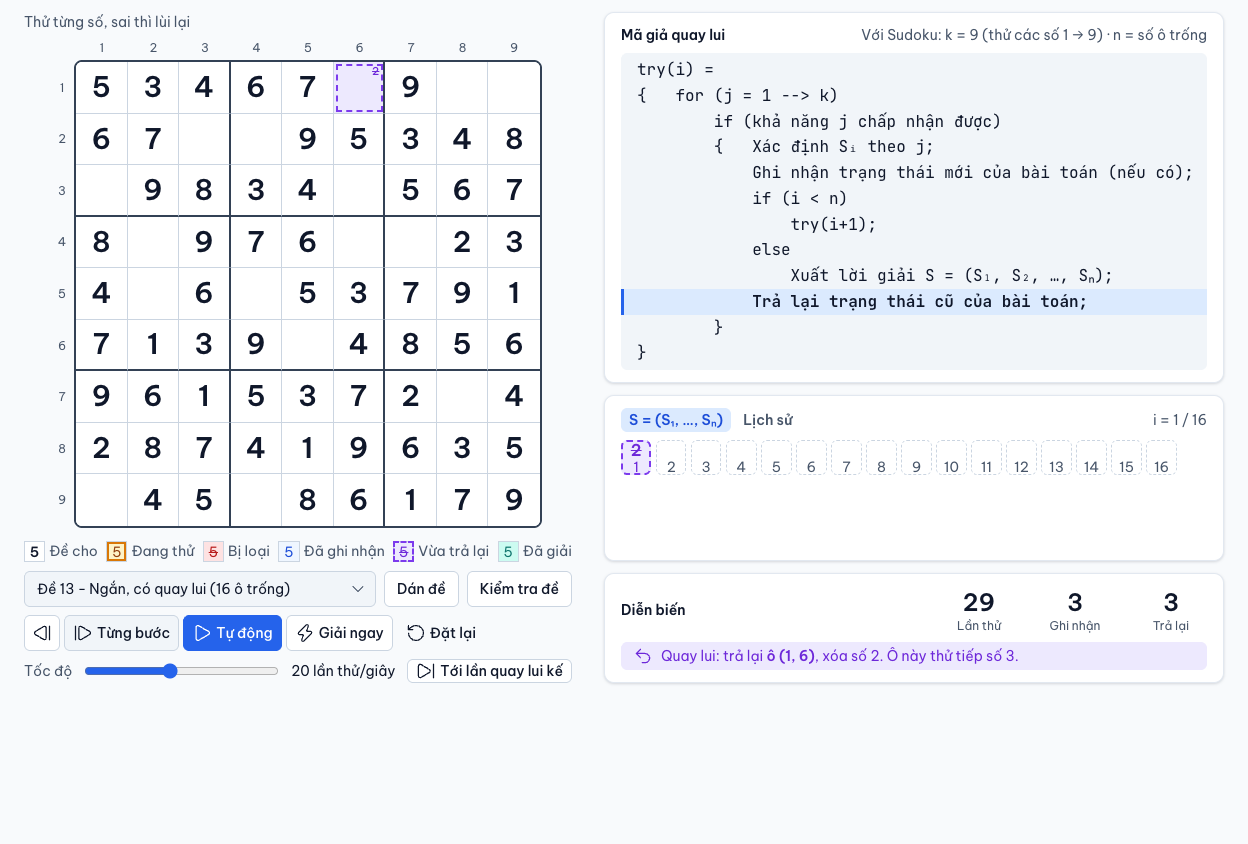
\includegraphics[width=0.95\linewidth]{figures/illustration-press-38.png}
  \caption{Lần bấm 38: thuật toán vừa trả lại ô (1, 6), xóa số 2. Bộ đếm: 29 lần thử, 3 ghi nhận, 3 trả lại}
  \label{fig:press-38}
\end{figure}

\subsection*{Giai đoạn 3: lần thử 30 đến 79, đi thẳng tới lời giải}

Ở ô \((1, 6)\), các số 3 đến 7 đều trùng hàng 1. Số 8 chấp nhận được ở lần thử 35. Từ đây thuật toán không quay lui lần nào nữa. Ô \((1, 8)\) nhận số 1, ô \((1, 9)\) nhận số 2, rồi 13 ô còn lại lần lượt nhận số. Ở lần thử 79 (lần bấm 118), ô trống cuối cùng \((9, 4)\) nhận số 2, và ở lần bấm 120 thuật toán xuất lời giải (Hình \ref{fig:press-120}).

\begin{figure}[H]
  \centering
  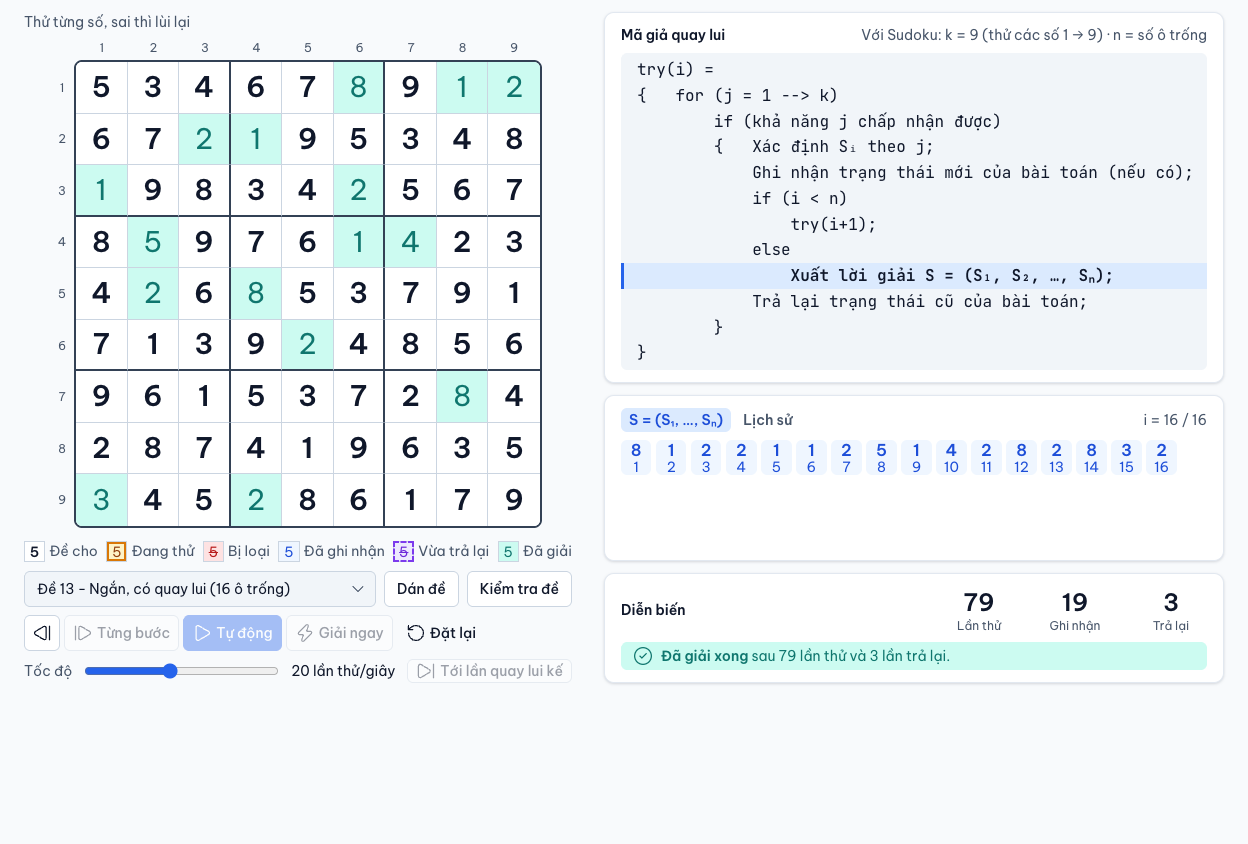
\includegraphics[width=0.95\linewidth]{figures/illustration-press-120.png}
  \caption{Lần bấm 120: đã giải xong. Bộ đếm: 79 lần thử, 19 ghi nhận, 3 trả lại}
  \label{fig:press-120}
\end{figure}

Kết quả cuối cùng là lời giải ở Hình \ref{fig:illustration-grids}(b), với \(S = (8, 1, 2, 2, 1, 1, 2, 5, 1, 4, 2, 8, 2, 8, 3, 2)\). Nếu không phải lùi lần nào, thuật toán chỉ cần thử \(S_1 + S_2 + \cdots + S_{16} = 52\) lần, vì ô thứ \(i\) thử từ 1 tới \(S_i\). Thực tế cần 79 lần, nên ba lần quay lui làm mất 27 lần thử, khoảng một phần ba tổng số. Thuật toán thử theo thứ tự cố định nên không ``nhìn'' trước như người giải bằng tay. Với cùng đề này, cách điền ô ít khả năng nhất trước (mục \ref{sec:variants}) chỉ cần 52 lần thử và không quay lui lần nào.

\section{Ví dụ thứ hai: quay lui qua sáu ô}
\label{sec:deep-example}

Ví dụ trên chỉ quay lui ở hàng 1. Đề mẫu số 3 ``Vừa'' có 40 ô trống, cần 1.909 lần thử và 187 lần trả lại, nên cho thấy một lần quay lui sâu hơn nhiều. Bảng \ref{tab:excerpt-steps} ghi các bước từ lần thử 783 đến lần thử 816, tức lần bấm 1.044 đến 1.089. Cột \(S_{13} \ldots S_{19}\) chỉ giữ bảy thành phần của vectơ \(S\) đang thay đổi trong đoạn này, vì đề có tới 40 thành phần.

Ở lần thử 704, thuật toán điền số 8 vào ô \((4, 1)\), tức \(S_{13} = 8\). Nhánh phía sau còn sống thêm 99 lần thử mới chết hẳn. Ở lần thử 783, ô \((5, 2)\) (\(i = 19\)) hết số: cả 9 số đều trùng. Từ đây thuật toán lùi liên tiếp qua sáu ô:

\begin{itemize}
  \item Ô \((5, 1)\) đang giữ 4. Các số 5 đến 9 đều trùng (lần thử 784 đến 788), nên thuật toán trả lại ô này.
  \item Ô \((4, 9)\) đang giữ 3. Các số 4 đến 9 đều trùng (lần thử 789 đến 794), nên trả lại tiếp.
  \item Ô \((4, 7)\) đang giữ 4. Các số 5 đến 9 đều trùng (lần thử 795 đến 799), nên trả lại tiếp.
  \item Ô \((4, 3)\) đang giữ 9, số cuối cùng, nên không còn số nào để thử. Thuật toán trả lại ngay, không tốn lần thử nào.
  \item Ô \((4, 2)\) đang giữ 5. Các số 6 đến 9 đều trùng (lần thử 800 đến 803), nên trả lại tiếp.
  \item Ô \((4, 1)\) đang giữ 8, số điền ở lần thử 704. Ở lần thử 803, thuật toán trả lại ô \((4, 1)\) (Hình \ref{fig:press-1070}) và thử tiếp số 9, được chấp nhận ở lần thử 804.
\end{itemize}

Sau đó thuật toán điền lại các ô phía sau. Ô \((4, 2)\) loại các số 1 đến 4 rồi nhận số 5 (lần thử 809). Ô \((4, 3)\) loại số 1 và 2 rồi nhận số 3 (lần thử 812). Ô \((4, 7)\) loại các số 1, 2 và 3 rồi nhận số 4 (lần thử 816). Số 8 mà ô \((4, 1)\) nhận ở lần thử 704 cũng nằm trong lời giải đầu tiên thuật toán tìm ra. Nhánh của nó chết vì trong các ô \(S_4\) đến \(S_{12}\) phía trước còn ô mang số khác với lời giải đó (\(S_4 = 2\) thay vì 7). Số 8 chỉ được điền lại ở lần thử 1.253, sau khi các ô đó đã đổi.

\begin{figure}[H]
  \centering
  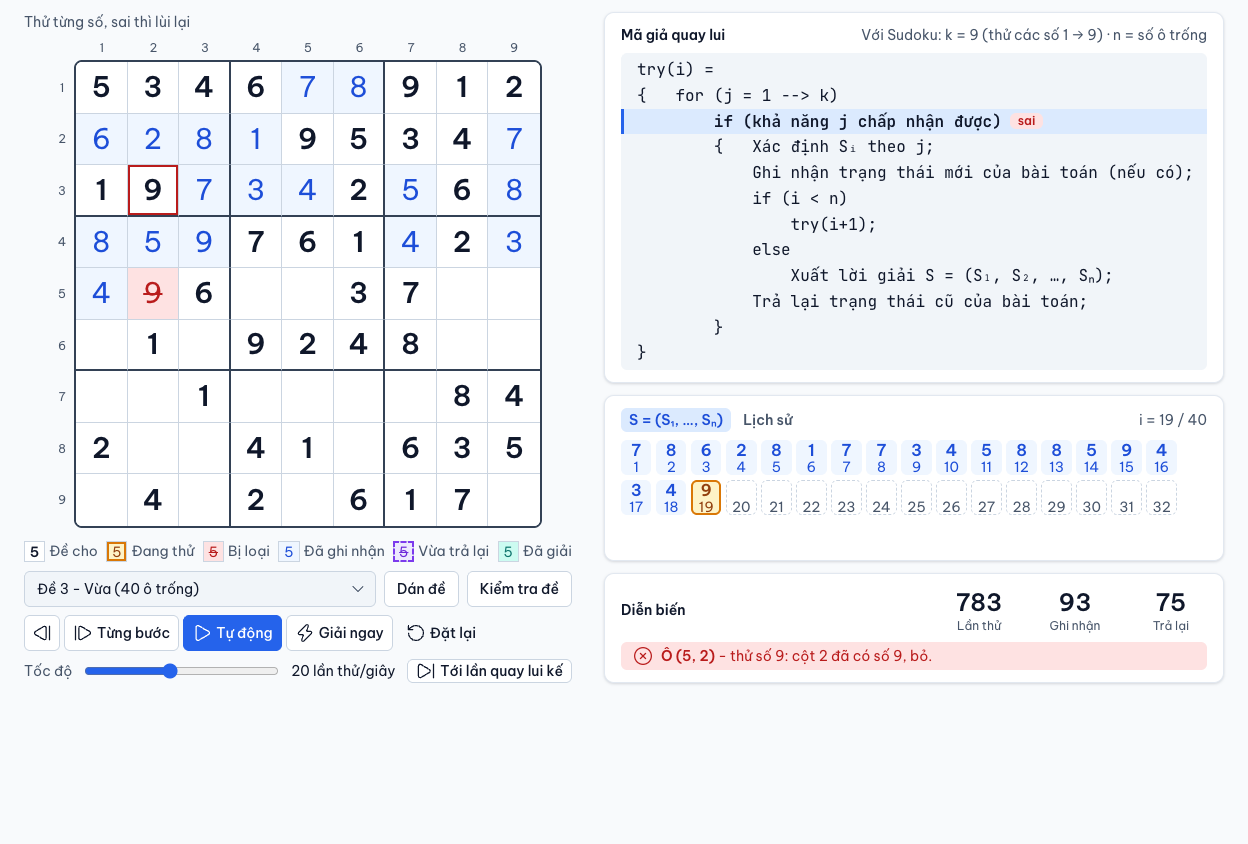
\includegraphics[width=0.85\linewidth]{figures/excerpt-press-1044.png}
  \caption{Lần bấm 1.044: ô \((5, 2)\) vừa hết số ở lần thử 783. Bộ đếm: 783 lần thử, 93 ghi nhận, 75 trả lại}
  \label{fig:press-1044}
\end{figure}

\begin{figure}[H]
  \centering
  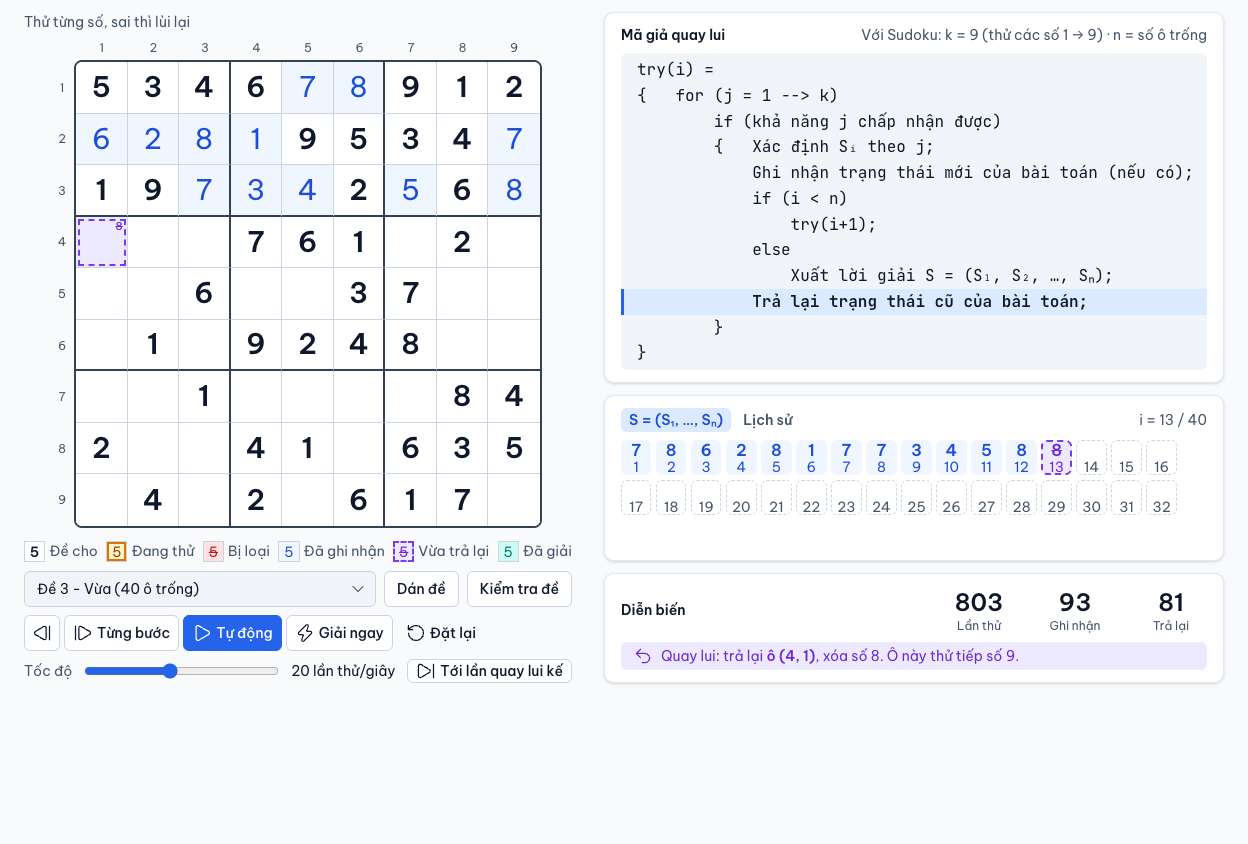
\includegraphics[width=0.85\linewidth]{figures/excerpt-press-1070.png}
  \caption{Lần bấm 1.070: thuật toán vừa trả lại ô \((4, 1)\), xóa số 8. Bộ đếm: 803 lần thử, 93 ghi nhận, 81 trả lại}
  \label{fig:press-1070}
\end{figure}

\begin{figure}[H]
  \centering
  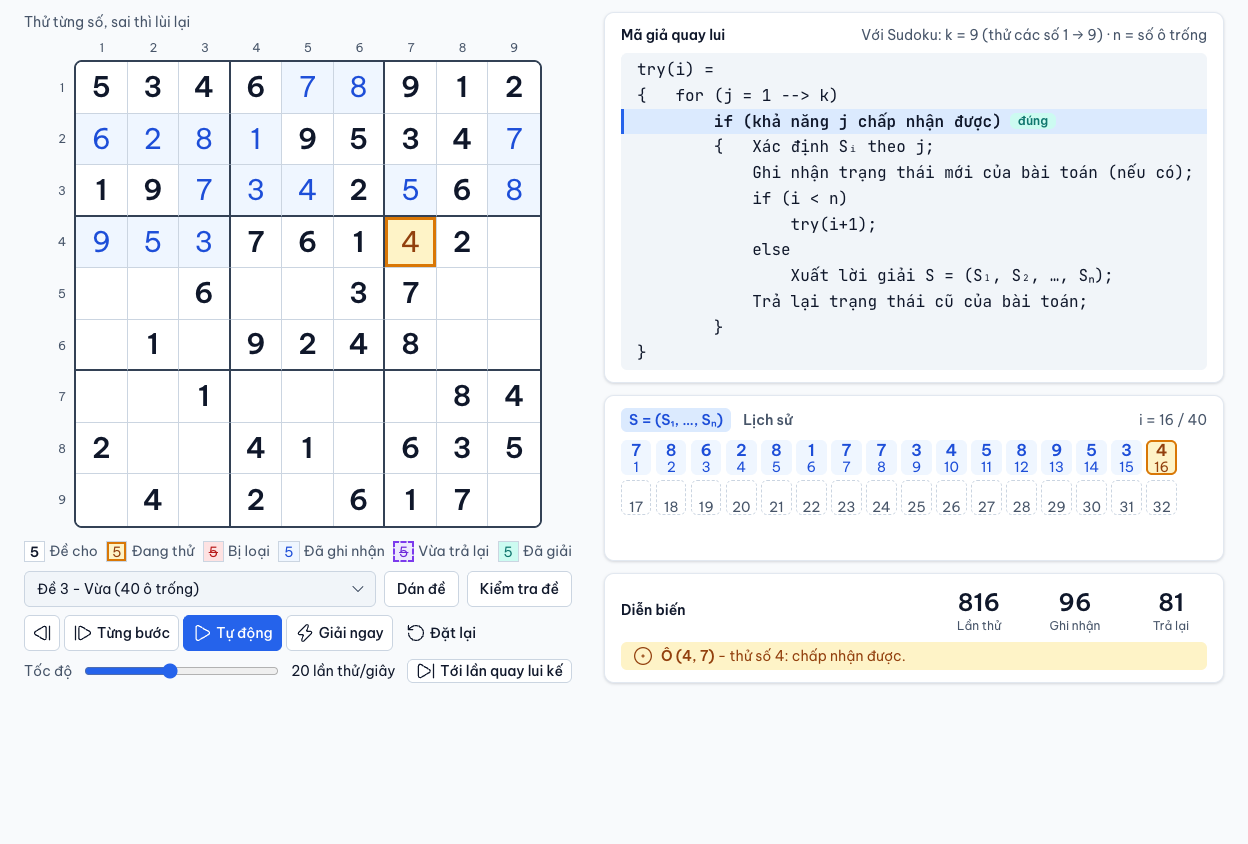
\includegraphics[width=0.85\linewidth]{figures/excerpt-press-1089.png}
  \caption{Lần bấm 1.089: ô \((4, 7)\) vừa nhận số 4 ở lần thử 816. Bộ đếm: 816 lần thử, 96 ghi nhận, 81 trả lại}
  \label{fig:press-1089}
\end{figure}

Muốn kiểm lại trên website, chọn đề 3 ``Vừa'' ở trang Giải Sudoku rồi bấm Từng bước đủ số lần ở cột Bấm. Nút ``Tới lần quay lui kế'' cho nhảy qua từng lần trả lại thay cho việc bấm tay hàng nghìn lần.

\begingroup\footnotesize\setlength{\tabcolsep}{3pt}
\begin{longtable}{@{}rrrcc>{\raggedright\arraybackslash}p{2.1cm}>{\raggedright\arraybackslash}p{3.7cm}>{\ttfamily}l@{}}
\caption{Các bước từ lần thử 783 đến lần thử 816 của đề ``Vừa''}\label{tab:excerpt-steps}\\
\toprule
\textbf{Bấm} & \textbf{Lần thử} & \(\boldsymbol{i}\) & \textbf{Ô} & \(\boldsymbol{j}\) & \textbf{Thao tác} & \textbf{Lý do} & \multicolumn{1}{l}{\textbf{\(S_{13} \ldots S_{19}\) sau bước}} \\
\midrule
\endfirsthead
\toprule
\textbf{Bấm} & \textbf{Lần thử} & \(\boldsymbol{i}\) & \textbf{Ô} & \(\boldsymbol{j}\) & \textbf{Thao tác} & \textbf{Lý do} & \multicolumn{1}{l}{\textbf{\(S_{13} \ldots S_{19}\) sau bước}} \\
\midrule
\endhead
\bottomrule
\endfoot
1044 & 783 & 19 & (5, 2) & 9 & Bị loại & trùng cột 2 ở ô (3, 2) & 8 5 9 4 3 4 . \\
1045 & 783 & 18 & (5, 1) & 4 & Trả lại & ô sau hết số & 8 5 9 4 3 . . \\
1046 & 784 & 18 & (5, 1) & 5 & Bị loại & trùng cột 1 ở ô (1, 1) & 8 5 9 4 3 . . \\
1047 & 785 & 18 & (5, 1) & 6 & Bị loại & trùng hàng 5 ở ô (5, 3) & 8 5 9 4 3 . . \\
1048 & 786 & 18 & (5, 1) & 7 & Bị loại & trùng hàng 5 ở ô (5, 7) & 8 5 9 4 3 . . \\
1049 & 787 & 18 & (5, 1) & 8 & Bị loại & trùng cột 1 ở ô (4, 1) & 8 5 9 4 3 . . \\
1050 & 788 & 18 & (5, 1) & 9 & Bị loại & trùng khối 4 ở ô (4, 3) & 8 5 9 4 3 . . \\
1051 & 788 & 17 & (4, 9) & 3 & Trả lại & ô sau hết số & 8 5 9 4 . . . \\
1052 & 789 & 17 & (4, 9) & 4 & Bị loại & trùng hàng 4 ở ô (4, 7) & 8 5 9 4 . . . \\
1053 & 790 & 17 & (4, 9) & 5 & Bị loại & trùng hàng 4 ở ô (4, 2) & 8 5 9 4 . . . \\
1054 & 791 & 17 & (4, 9) & 6 & Bị loại & trùng hàng 4 ở ô (4, 5) & 8 5 9 4 . . . \\
1055 & 792 & 17 & (4, 9) & 7 & Bị loại & trùng hàng 4 ở ô (4, 4) & 8 5 9 4 . . . \\
1056 & 793 & 17 & (4, 9) & 8 & Bị loại & trùng hàng 4 ở ô (4, 1) & 8 5 9 4 . . . \\
1057 & 794 & 17 & (4, 9) & 9 & Bị loại & trùng hàng 4 ở ô (4, 3) & 8 5 9 4 . . . \\
1058 & 794 & 16 & (4, 7) & 4 & Trả lại & ô sau hết số & 8 5 9 . . . . \\
1059 & 795 & 16 & (4, 7) & 5 & Bị loại & trùng hàng 4 ở ô (4, 2) & 8 5 9 . . . . \\
1060 & 796 & 16 & (4, 7) & 6 & Bị loại & trùng hàng 4 ở ô (4, 5) & 8 5 9 . . . . \\
1061 & 797 & 16 & (4, 7) & 7 & Bị loại & trùng hàng 4 ở ô (4, 4) & 8 5 9 . . . . \\
1062 & 798 & 16 & (4, 7) & 8 & Bị loại & trùng hàng 4 ở ô (4, 1) & 8 5 9 . . . . \\
1063 & 799 & 16 & (4, 7) & 9 & Bị loại & trùng hàng 4 ở ô (4, 3) & 8 5 9 . . . . \\
1064 & 799 & 15 & (4, 3) & 9 & Trả lại & ô sau hết số & 8 5 . . . . . \\
1065 & 799 & 14 & (4, 2) & 5 & Trả lại & ô sau hết số & 8 . . . . . . \\
1066 & 800 & 14 & (4, 2) & 6 & Bị loại & trùng hàng 4 ở ô (4, 5) & 8 . . . . . . \\
1067 & 801 & 14 & (4, 2) & 7 & Bị loại & trùng hàng 4 ở ô (4, 4) & 8 . . . . . . \\
1068 & 802 & 14 & (4, 2) & 8 & Bị loại & trùng hàng 4 ở ô (4, 1) & 8 . . . . . . \\
1069 & 803 & 14 & (4, 2) & 9 & Bị loại & trùng cột 2 ở ô (3, 2) & 8 . . . . . . \\
1070 & 803 & 13 & (4, 1) & 8 & Trả lại & ô sau hết số & . . . . . . . \\
1071 & 804 & 13 & (4, 1) & 9 & Chấp nhận & không trùng & 9 . . . . . . \\
1074 & 805 & 14 & (4, 2) & 1 & Bị loại & trùng hàng 4 ở ô (4, 6) & 9 . . . . . . \\
1075 & 806 & 14 & (4, 2) & 2 & Bị loại & trùng hàng 4 ở ô (4, 8) & 9 . . . . . . \\
1076 & 807 & 14 & (4, 2) & 3 & Bị loại & trùng cột 2 ở ô (1, 2) & 9 . . . . . . \\
1077 & 808 & 14 & (4, 2) & 4 & Bị loại & trùng cột 2 ở ô (9, 2) & 9 . . . . . . \\
1078 & 809 & 14 & (4, 2) & 5 & Chấp nhận & không trùng & 9 5 . . . . . \\
1081 & 810 & 15 & (4, 3) & 1 & Bị loại & trùng hàng 4 ở ô (4, 6) & 9 5 . . . . . \\
1082 & 811 & 15 & (4, 3) & 2 & Bị loại & trùng hàng 4 ở ô (4, 8) & 9 5 . . . . . \\
1083 & 812 & 15 & (4, 3) & 3 & Chấp nhận & không trùng & 9 5 3 . . . . \\
1086 & 813 & 16 & (4, 7) & 1 & Bị loại & trùng hàng 4 ở ô (4, 6) & 9 5 3 . . . . \\
1087 & 814 & 16 & (4, 7) & 2 & Bị loại & trùng hàng 4 ở ô (4, 8) & 9 5 3 . . . . \\
1088 & 815 & 16 & (4, 7) & 3 & Bị loại & trùng hàng 4 ở ô (4, 3) & 9 5 3 . . . . \\
1089 & 816 & 16 & (4, 7) & 4 & Chấp nhận & không trùng & 9 5 3 4 . . . \\
\end{longtable}
\endgroup


\section{Bảng toàn bộ các bước}

\begingroup\footnotesize\setlength{\tabcolsep}{3pt}
\begin{longtable}{@{}rrrcc>{\raggedright\arraybackslash}p{2.1cm}>{\raggedright\arraybackslash}p{3.3cm}>{\ttfamily}l@{}}
\caption{Toàn bộ các bước giải đề số 13}\label{tab:illustration-steps}\\
\toprule
\textbf{Bấm} & \textbf{Lần thử} & \(\boldsymbol{i}\) & \textbf{Ô} & \(\boldsymbol{j}\) & \textbf{Thao tác} & \textbf{Lý do} & \multicolumn{1}{l}{\textbf{\(S\) sau bước}} \\
\midrule
\endfirsthead
\toprule
\textbf{Bấm} & \textbf{Lần thử} & \(\boldsymbol{i}\) & \textbf{Ô} & \(\boldsymbol{j}\) & \textbf{Thao tác} & \textbf{Lý do} & \multicolumn{1}{l}{\textbf{\(S\) sau bước}} \\
\midrule
\endhead
\bottomrule
\endfoot
1 & 1 & 1 & (1, 6) & 1 & Chấp nhận & không trùng & 1 . . . . . . . . . . . . . . . \\
4 & 2 & 2 & (1, 8) & 1 & Bị loại & trùng hàng 1 ở ô (1, 6) & 1 . . . . . . . . . . . . . . . \\
5 & 3 & 2 & (1, 8) & 2 & Bị loại & trùng cột 8 ở ô (4, 8) & 1 . . . . . . . . . . . . . . . \\
6 & 4 & 2 & (1, 8) & 3 & Bị loại & trùng hàng 1 ở ô (1, 2) & 1 . . . . . . . . . . . . . . . \\
7 & 5 & 2 & (1, 8) & 4 & Bị loại & trùng hàng 1 ở ô (1, 3) & 1 . . . . . . . . . . . . . . . \\
8 & 6 & 2 & (1, 8) & 5 & Bị loại & trùng hàng 1 ở ô (1, 1) & 1 . . . . . . . . . . . . . . . \\
9 & 7 & 2 & (1, 8) & 6 & Bị loại & trùng hàng 1 ở ô (1, 4) & 1 . . . . . . . . . . . . . . . \\
10 & 8 & 2 & (1, 8) & 7 & Bị loại & trùng hàng 1 ở ô (1, 5) & 1 . . . . . . . . . . . . . . . \\
11 & 9 & 2 & (1, 8) & 8 & Bị loại & trùng khối 3 ở ô (2, 9) & 1 . . . . . . . . . . . . . . . \\
12 & 10 & 2 & (1, 8) & 9 & Bị loại & trùng hàng 1 ở ô (1, 7) & 1 . . . . . . . . . . . . . . . \\
13 & 10 & 1 & (1, 6) & 1 & Trả lại & ô sau hết số & . . . . . . . . . . . . . . . . \\
14 & 11 & 1 & (1, 6) & 2 & Chấp nhận & không trùng & 2 . . . . . . . . . . . . . . . \\
17 & 12 & 2 & (1, 8) & 1 & Chấp nhận & không trùng & 2 1 . . . . . . . . . . . . . . \\
20 & 13 & 3 & (1, 9) & 1 & Bị loại & trùng hàng 1 ở ô (1, 8) & 2 1 . . . . . . . . . . . . . . \\
21 & 14 & 3 & (1, 9) & 2 & Bị loại & trùng hàng 1 ở ô (1, 6) & 2 1 . . . . . . . . . . . . . . \\
22 & 15 & 3 & (1, 9) & 3 & Bị loại & trùng hàng 1 ở ô (1, 2) & 2 1 . . . . . . . . . . . . . . \\
23 & 16 & 3 & (1, 9) & 4 & Bị loại & trùng hàng 1 ở ô (1, 3) & 2 1 . . . . . . . . . . . . . . \\
24 & 17 & 3 & (1, 9) & 5 & Bị loại & trùng hàng 1 ở ô (1, 1) & 2 1 . . . . . . . . . . . . . . \\
25 & 18 & 3 & (1, 9) & 6 & Bị loại & trùng hàng 1 ở ô (1, 4) & 2 1 . . . . . . . . . . . . . . \\
26 & 19 & 3 & (1, 9) & 7 & Bị loại & trùng hàng 1 ở ô (1, 5) & 2 1 . . . . . . . . . . . . . . \\
27 & 20 & 3 & (1, 9) & 8 & Bị loại & trùng cột 9 ở ô (2, 9) & 2 1 . . . . . . . . . . . . . . \\
28 & 21 & 3 & (1, 9) & 9 & Bị loại & trùng hàng 1 ở ô (1, 7) & 2 1 . . . . . . . . . . . . . . \\
29 & 21 & 2 & (1, 8) & 1 & Trả lại & ô sau hết số & 2 . . . . . . . . . . . . . . . \\
30 & 22 & 2 & (1, 8) & 2 & Bị loại & trùng hàng 1 ở ô (1, 6) & 2 . . . . . . . . . . . . . . . \\
31 & 23 & 2 & (1, 8) & 3 & Bị loại & trùng hàng 1 ở ô (1, 2) & 2 . . . . . . . . . . . . . . . \\
32 & 24 & 2 & (1, 8) & 4 & Bị loại & trùng hàng 1 ở ô (1, 3) & 2 . . . . . . . . . . . . . . . \\
33 & 25 & 2 & (1, 8) & 5 & Bị loại & trùng hàng 1 ở ô (1, 1) & 2 . . . . . . . . . . . . . . . \\
34 & 26 & 2 & (1, 8) & 6 & Bị loại & trùng hàng 1 ở ô (1, 4) & 2 . . . . . . . . . . . . . . . \\
35 & 27 & 2 & (1, 8) & 7 & Bị loại & trùng hàng 1 ở ô (1, 5) & 2 . . . . . . . . . . . . . . . \\
36 & 28 & 2 & (1, 8) & 8 & Bị loại & trùng khối 3 ở ô (2, 9) & 2 . . . . . . . . . . . . . . . \\
37 & 29 & 2 & (1, 8) & 9 & Bị loại & trùng hàng 1 ở ô (1, 7) & 2 . . . . . . . . . . . . . . . \\
38 & 29 & 1 & (1, 6) & 2 & Trả lại & ô sau hết số & . . . . . . . . . . . . . . . . \\
39 & 30 & 1 & (1, 6) & 3 & Bị loại & trùng hàng 1 ở ô (1, 2) & . . . . . . . . . . . . . . . . \\
40 & 31 & 1 & (1, 6) & 4 & Bị loại & trùng hàng 1 ở ô (1, 3) & . . . . . . . . . . . . . . . . \\
41 & 32 & 1 & (1, 6) & 5 & Bị loại & trùng hàng 1 ở ô (1, 1) & . . . . . . . . . . . . . . . . \\
42 & 33 & 1 & (1, 6) & 6 & Bị loại & trùng hàng 1 ở ô (1, 4) & . . . . . . . . . . . . . . . . \\
43 & 34 & 1 & (1, 6) & 7 & Bị loại & trùng hàng 1 ở ô (1, 5) & . . . . . . . . . . . . . . . . \\
44 & 35 & 1 & (1, 6) & 8 & Chấp nhận & không trùng & 8 . . . . . . . . . . . . . . . \\
47 & 36 & 2 & (1, 8) & 1 & Chấp nhận & không trùng & 8 1 . . . . . . . . . . . . . . \\
50 & 37 & 3 & (1, 9) & 1 & Bị loại & trùng hàng 1 ở ô (1, 8) & 8 1 . . . . . . . . . . . . . . \\
51 & 38 & 3 & (1, 9) & 2 & Chấp nhận & không trùng & 8 1 2 . . . . . . . . . . . . . \\
54 & 39 & 4 & (2, 3) & 1 & Bị loại & trùng cột 3 ở ô (7, 3) & 8 1 2 . . . . . . . . . . . . . \\
55 & 40 & 4 & (2, 3) & 2 & Chấp nhận & không trùng & 8 1 2 2 . . . . . . . . . . . . \\
58 & 41 & 5 & (2, 4) & 1 & Chấp nhận & không trùng & 8 1 2 2 1 . . . . . . . . . . . \\
61 & 42 & 6 & (3, 1) & 1 & Chấp nhận & không trùng & 8 1 2 2 1 1 . . . . . . . . . . \\
64 & 43 & 7 & (3, 6) & 1 & Bị loại & trùng hàng 3 ở ô (3, 1) & 8 1 2 2 1 1 . . . . . . . . . . \\
65 & 44 & 7 & (3, 6) & 2 & Chấp nhận & không trùng & 8 1 2 2 1 1 2 . . . . . . . . . \\
68 & 45 & 8 & (4, 2) & 1 & Bị loại & trùng cột 2 ở ô (6, 2) & 8 1 2 2 1 1 2 . . . . . . . . . \\
69 & 46 & 8 & (4, 2) & 2 & Bị loại & trùng hàng 4 ở ô (4, 8) & 8 1 2 2 1 1 2 . . . . . . . . . \\
70 & 47 & 8 & (4, 2) & 3 & Bị loại & trùng hàng 4 ở ô (4, 9) & 8 1 2 2 1 1 2 . . . . . . . . . \\
71 & 48 & 8 & (4, 2) & 4 & Bị loại & trùng cột 2 ở ô (9, 2) & 8 1 2 2 1 1 2 . . . . . . . . . \\
72 & 49 & 8 & (4, 2) & 5 & Chấp nhận & không trùng & 8 1 2 2 1 1 2 5 . . . . . . . . \\
75 & 50 & 9 & (4, 6) & 1 & Chấp nhận & không trùng & 8 1 2 2 1 1 2 5 1 . . . . . . . \\
78 & 51 & 10 & (4, 7) & 1 & Bị loại & trùng hàng 4 ở ô (4, 6) & 8 1 2 2 1 1 2 5 1 . . . . . . . \\
79 & 52 & 10 & (4, 7) & 2 & Bị loại & trùng hàng 4 ở ô (4, 8) & 8 1 2 2 1 1 2 5 1 . . . . . . . \\
80 & 53 & 10 & (4, 7) & 3 & Bị loại & trùng hàng 4 ở ô (4, 9) & 8 1 2 2 1 1 2 5 1 . . . . . . . \\
81 & 54 & 10 & (4, 7) & 4 & Chấp nhận & không trùng & 8 1 2 2 1 1 2 5 1 4 . . . . . . \\
84 & 55 & 11 & (5, 2) & 1 & Bị loại & trùng hàng 5 ở ô (5, 9) & 8 1 2 2 1 1 2 5 1 4 . . . . . . \\
85 & 56 & 11 & (5, 2) & 2 & Chấp nhận & không trùng & 8 1 2 2 1 1 2 5 1 4 2 . . . . . \\
88 & 57 & 12 & (5, 4) & 1 & Bị loại & trùng hàng 5 ở ô (5, 9) & 8 1 2 2 1 1 2 5 1 4 2 . . . . . \\
89 & 58 & 12 & (5, 4) & 2 & Bị loại & trùng hàng 5 ở ô (5, 2) & 8 1 2 2 1 1 2 5 1 4 2 . . . . . \\
90 & 59 & 12 & (5, 4) & 3 & Bị loại & trùng hàng 5 ở ô (5, 6) & 8 1 2 2 1 1 2 5 1 4 2 . . . . . \\
91 & 60 & 12 & (5, 4) & 4 & Bị loại & trùng hàng 5 ở ô (5, 1) & 8 1 2 2 1 1 2 5 1 4 2 . . . . . \\
92 & 61 & 12 & (5, 4) & 5 & Bị loại & trùng hàng 5 ở ô (5, 5) & 8 1 2 2 1 1 2 5 1 4 2 . . . . . \\
93 & 62 & 12 & (5, 4) & 6 & Bị loại & trùng hàng 5 ở ô (5, 3) & 8 1 2 2 1 1 2 5 1 4 2 . . . . . \\
94 & 63 & 12 & (5, 4) & 7 & Bị loại & trùng hàng 5 ở ô (5, 7) & 8 1 2 2 1 1 2 5 1 4 2 . . . . . \\
95 & 64 & 12 & (5, 4) & 8 & Chấp nhận & không trùng & 8 1 2 2 1 1 2 5 1 4 2 8 . . . . \\
98 & 65 & 13 & (6, 5) & 1 & Bị loại & trùng hàng 6 ở ô (6, 2) & 8 1 2 2 1 1 2 5 1 4 2 8 . . . . \\
99 & 66 & 13 & (6, 5) & 2 & Chấp nhận & không trùng & 8 1 2 2 1 1 2 5 1 4 2 8 2 . . . \\
102 & 67 & 14 & (7, 8) & 1 & Bị loại & trùng hàng 7 ở ô (7, 3) & 8 1 2 2 1 1 2 5 1 4 2 8 2 . . . \\
103 & 68 & 14 & (7, 8) & 2 & Bị loại & trùng hàng 7 ở ô (7, 7) & 8 1 2 2 1 1 2 5 1 4 2 8 2 . . . \\
104 & 69 & 14 & (7, 8) & 3 & Bị loại & trùng hàng 7 ở ô (7, 5) & 8 1 2 2 1 1 2 5 1 4 2 8 2 . . . \\
105 & 70 & 14 & (7, 8) & 4 & Bị loại & trùng hàng 7 ở ô (7, 9) & 8 1 2 2 1 1 2 5 1 4 2 8 2 . . . \\
106 & 71 & 14 & (7, 8) & 5 & Bị loại & trùng hàng 7 ở ô (7, 4) & 8 1 2 2 1 1 2 5 1 4 2 8 2 . . . \\
107 & 72 & 14 & (7, 8) & 6 & Bị loại & trùng hàng 7 ở ô (7, 2) & 8 1 2 2 1 1 2 5 1 4 2 8 2 . . . \\
108 & 73 & 14 & (7, 8) & 7 & Bị loại & trùng hàng 7 ở ô (7, 6) & 8 1 2 2 1 1 2 5 1 4 2 8 2 . . . \\
109 & 74 & 14 & (7, 8) & 8 & Chấp nhận & không trùng & 8 1 2 2 1 1 2 5 1 4 2 8 2 8 . . \\
112 & 75 & 15 & (9, 1) & 1 & Bị loại & trùng hàng 9 ở ô (9, 7) & 8 1 2 2 1 1 2 5 1 4 2 8 2 8 . . \\
113 & 76 & 15 & (9, 1) & 2 & Bị loại & trùng cột 1 ở ô (8, 1) & 8 1 2 2 1 1 2 5 1 4 2 8 2 8 . . \\
114 & 77 & 15 & (9, 1) & 3 & Chấp nhận & không trùng & 8 1 2 2 1 1 2 5 1 4 2 8 2 8 3 . \\
117 & 78 & 16 & (9, 4) & 1 & Bị loại & trùng hàng 9 ở ô (9, 7) & 8 1 2 2 1 1 2 5 1 4 2 8 2 8 3 . \\
118 & 79 & 16 & (9, 4) & 2 & Chấp nhận & không trùng & 8 1 2 2 1 1 2 5 1 4 2 8 2 8 3 2 \\
120 & 79 &  &  &  & Có lời giải & đủ 16 ô & 8 1 2 2 1 1 2 5 1 4 2 8 2 8 3 2 \\
\end{longtable}
\endgroup


\chapter{Quá trình thiết kế và xây dựng}

Em dùng Claude Code để lập kế hoạch, viết code, viết test và đo đạc. Phần chọn hướng, duyệt kết quả và quyết định cuối cùng do em giữ. Chương này kể lại từng giai đoạn theo thứ tự thời gian, từ ngày 3/10 đến ngày 12/10/2026.

Nguồn của chương là nhật ký làm việc \texttt{work-log.md}, em ghi ngay sau mỗi buổi, và transcript của Claude Code lưu trên máy. Mọi prompt trong chương chép nguyên văn từ transcript, kể cả lỗi chính tả. Mỗi giai đoạn ghi công cụ, prompt, kết quả, vấn đề gặp phải và cách em kiểm chứng.

\section{Công cụ và cách làm việc}

Bảng \ref{tab:tools} liệt kê các công cụ, thư viện và model em dùng.

\begin{table}[H]
  \centering
  \caption{Công cụ, thư viện và model}
  \label{tab:tools}
  \begin{tabularx}{\linewidth}{@{}>{\raggedright\arraybackslash}p{5.2cm}L@{}}
    \toprule
    \textbf{Công cụ} & \textbf{Vai trò} \\
    \midrule
    Claude Code (tiện ích VS Code, phiên bản 2.1.287 đến 2.1.295), model Claude Opus 5.5 & Lập kế hoạch, viết code website và các script, viết test, đo đạc, mở website trên Chrome để chụp màn hình và tự soát, viết nháp chữ trên website và report \\
    Claude Design (trên claude.ai) & Vẽ 19 khung hình giao diện từ một prompt do Claude Code soạn \\
    Một phiên Claude Code riêng & Đóng vai người dùng phổ thông, nhận xét website \\
    React 19, React Router 8, TypeScript 6, Vite 8 & Website chạy hoàn toàn trên trình duyệt, không có máy chủ \\
    Vitest 5, Playwright 1.63, oxlint & Test đơn vị, test trên Chrome thật, soát lỗi code \\
    Python 3.9 & Các bản cài đặt tham chiếu để đối chiếu, script sinh bộ testcase \\
    Yarn 4.18.1, lucide-react, Fontsource & Quản lý gói, biểu tượng, phông Be Vietnam Pro và JetBrains Mono \\
    XeLaTeX & Report này \\
    \bottomrule
  \end{tabularx}
\end{table}

Mỗi việc đi qua cùng một vòng:

\begin{itemize}
  \item Em nêu yêu cầu bằng một prompt ngắn.
  \item Claude đọc code hiện có, đo đạc khi cần, rồi đề xuất phương án. Chỗ nào có nhiều lựa chọn thì Claude hỏi lại em.
  \item Em chọn. Claude làm, chạy test, mở website trên Chrome thật để chụp màn hình và tự soát.
  \item Em xem kết quả, góp ý tiếp, rồi ghi vào nhật ký.
\end{itemize}

Ngay prompt lập kế hoạch đầu tiên, em đặt luật văn phong cho Claude. Em giữ nguyên bảy dòng tiếng Anh:

\begin{promptbox}{3/10, kèm theo prompt lập kế hoạch}
- Cut hype, buzzwords, empty phrasing and anything that reads like marketing copy.\\
- Write with a clear position. Fewer “it depends” hedges, fewer generic recommendations.\\
- Mix short, medium and long sentences. Uniform, too-perfect rhythm reads as machine-written.\\
- Replace vague claims with examples, scenarios and real detail — numbers, file paths, commit hashes.\\
- Use plain, natural words, as if explaining to someone without much background in the topic.\\
- Drop generic openers, filler, repeated transitions and summary paragraphs that add nothing.\\
- Match the user's own voice: sample a few things they wrote, then follow that word choice, sentence rhythm and personality.
\end{promptbox}

Luật về code em đặt ngay sau đó, và giữ suốt dự án:

\begin{promptbox}{3/10}
Remember everything in code should be in English, code must be easy to read, easy to understand, must be explicit, can explain itself without comment. Do you think we can use React for the website?
\end{promptbox}

\section{Chọn đề và lập kế hoạch (3/10)}

Em phân vân giữa Dijkstra và Sudoku.

\begin{promptbox}{3/10}
Bạn nghĩ sao về Dijkstra, tôi cũng thích Sudoku
\end{promptbox}

Claude khuyên bỏ Dijkstra vì trên lớp chưa học, cô chỉ nhắc tới như bài của khóa trước. Em chọn Sudoku. Lý do: em đã tự cài đặt quay lui theo mô hình 1 cho bài này từ trước, và bài toán có đủ ba động tác thử, loại, quay lui để nhìn thấy trên hình.

Em yêu cầu lập kế hoạch đầy đủ trước khi viết dòng code nào:

\begin{promptbox}{3/10}
Ok, tôi đồng ý với Sudoku, nhưng chúng ta sẽ không thực hiện liền mà cần lên kế hoạch phân tích toàn bộ bài toán trước khi viết những dòng code đầu tiên. Vì vậy, hãy tạo 1 file markdown chứa toàn bộ chi tiết kế hoạch cho bài tập lớn này, lưu ý, giọng văn của bạn phải tuân thủ tuyệt đối theo yêu cầu của tôi dưới đây [bảy dòng luật văn phong ở mục trên]
\end{promptbox}

Claude viết \texttt{plan.md} gồm 12 mục. Trước khi viết, Claude chạy bản cài đặt Python của em trên 7 đề để lấy số đo thật. Các quyết định thiết kế dựa vào số đo đó. Đề Arto Inkala cần 445.778 lần thử, nên không thể chỉ có hoạt ảnh chậm: website phải có thêm nút giải một mạch.

\begin{promptbox}{3/10}
5.1. I wanna build a completely website and deploy to Netlify or any supported free server\\
6. UI must be nice, modern, can I use Claude Design for this?
\end{promptbox}

\begin{promptbox}{3/10}
Yes, file name should be in English as well. Don't need to care about zip and offline for now. Just let me know if we use React, does it affect to the performance?
\end{promptbox}

Câu hỏi hiệu năng có câu trả lời bằng số đo. Trên đề Inkala, bản đệ quy thường chạy hết 3,7 ms. Bản viết thành generator, để giao diện dừng được ở từng bước, mất 623 ms. Phần chậm nằm ở generator, không nằm ở React. Từ số đo này, kế hoạch chốt cách vẽ: mỗi khung hình lấy một loạt bước rồi mới vẽ lại một lần, thay vì vẽ lại sau từng bước.

\section{Thiết kế giao diện bằng Claude Design (3/10 - 4/10)}

\begin{promptbox}{3/10}
Can we build a very detail prompt then I can use to talk with Claude Design for the mockup? We should have the color pallet for the website, it should be mordern, no violate design rule.
\end{promptbox}

Claude Code soạn file \texttt{design/claude-design-prompt.md}. File này có bốn điểm em thấy quan trọng:

\begin{itemize}
  \item \textbf{Bảng màu có đo độ tương phản} theo chuẩn WCAG AA. Một màu xám chỉ đạt 4,34:1, thiếu so với mức 4,5:1, nên Claude bỏ màu đó.
  \item \textbf{Mỗi trạng thái ô có dấu hiệu ngoài màu}, ví dụ số không hợp lệ có thêm nét gạch ngang, để người khó phân biệt đỏ và xanh vẫn đọc được.
  \item \textbf{Trạng thái lưới lấy từ lần chạy thật} của đề ``Vừa'' tại lần thử 803, lần thử 814 và lúc giải xong, không vẽ phỏng đoán.
  \item \textbf{Mã giả chép đúng từng chữ slide} mô hình 1 của cô.
\end{itemize}

Em đưa prompt vào Claude Design và trong lúc làm yêu cầu thêm nút chuyển Sáng và Tối. Claude Design trả về 19 khung hình, file màu \texttt{tokens.css} và hướng dẫn bàn giao. Hình \ref{fig:design-frame} là một khung trong số đó.

\begin{figure}[H]
  \centering
  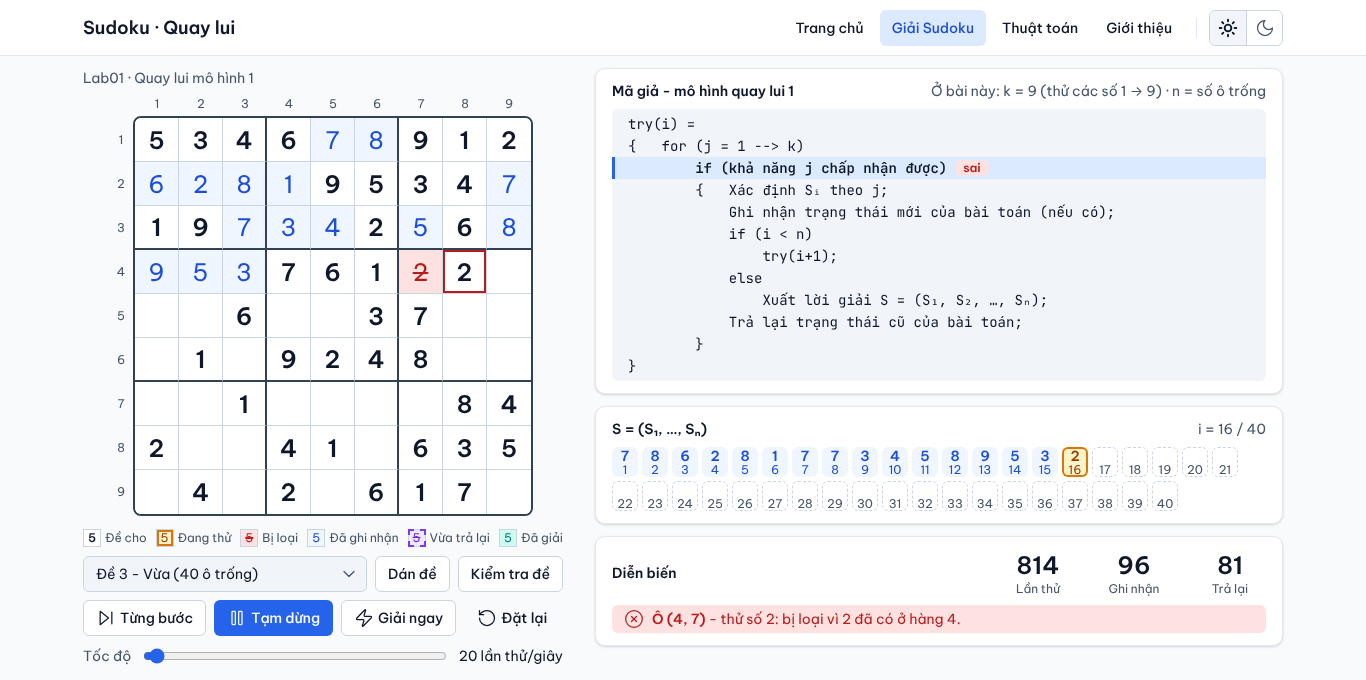
\includegraphics[width=0.92\linewidth]{figures/design-frame-04-rejected.png}
  \caption{Khung 04 của bản thiết kế: lần thử 814 của đề ``Vừa'', số 2 bị loại ở ô (4, 7)}
  \label{fig:design-frame}
\end{figure}

\begin{promptbox}{4/10}
Claude Design has finished their job and hand-off design in the folder design, you can take a look at this and let me know what your plan next?
\end{promptbox}

Trước khi code theo bản thiết kế, Claude chạy lại thuật toán tới đúng thời điểm của từng khung để soát số. Khung 04 (lần thử 814), khung 05 (lần thử 803) và khung 17 (đề Inkala ở lần thử 200.000) đều khớp từng con số.

\section{Chuyển thuật toán sang TypeScript (4/10)}

Claude viết lại bản cài đặt của em bằng TypeScript, đặt trong thư mục \texttt{website/src/solver}. Hàm \texttt{tryStep(i)} giữ đúng các bước của mô hình 1. Khác biệt duy nhất: ở mỗi bước, hàm phát ra một sự kiện để giao diện vẽ. Bảng đối chiếu từng dòng nằm ở Chương 4.

Đáp án cho test là bản Python thêm ba bộ đếm: số lần thử, số lần ghi nhận, số lần trả lại. Hai bản phải cho cùng lời giải và cùng ba con số trên mọi đề. Lần đầu có 29 test, tất cả đạt.

Tất cả đạt ngay lần đầu chưa chứng minh được gì, nên Claude thử làm sai thuật toán xem test có bắt được không:

\begin{itemize}
  \item \textbf{Bỏ số 9} khỏi vòng thử: 10 test báo lỗi.
  \item \textbf{Kiểm tra cột trước hàng}: không test nào báo lỗi. Lý do: ba thời điểm chụp dùng làm đáp án đều chỉ trùng ở hàng. Claude thêm một test duyệt toàn bộ 1.682 lần bị loại của đề ``Vừa'', so cả lý do bị loại. Từ đó test bắt được lỗi này.
\end{itemize}

Giai đoạn này có hai sự cố nhỏ với trình quản lý gói:

\begin{promptbox}{4/10}
Can we use yarn v2 instead of npm?
\end{promptbox}

\begin{itemize}
  \item Yarn 2 đã ngừng hỗ trợ, nên Claude dùng Yarn 4.18.1, cùng kiến trúc với bản 2. Lần chạy đầu, Yarn ghi nhầm ba file vào thư mục home vì ở đó có một file \texttt{yarn.lock} rỗng từ ngày 26/8. Claude xóa đúng ba thứ vừa tạo, giữ nguyên file cũ, rồi chạy lại trong thư mục dự án.
  \item Yarn 4 từ chối cài lucide-react 1.51.0 vì bản này phát hành chưa đủ 24 giờ. Claude giữ lớp bảo vệ đó và dùng bản 1.50.0.
\end{itemize}

\section{Xây dựng trang Giải Sudoku (4/10)}

Website lúc đầu còn ghi chữ ``Wecode'' trên giao diện. Em yêu cầu bỏ:

\begin{promptbox}{4/10}
Yes, please go head. But before moving forward, I don't think label “Wecode” is ok, we can use another label, right?
\end{promptbox}

\begin{promptbox}{4/10}
I mean don't want any text relates to “Lab” “Wecode” like we're studying. Treat this website like the one to be used for people understand the algorithm, not my exercises
\end{promptbox}

Từ đây website viết cho người muốn hiểu thuật toán. Mã giả vẫn chép đúng slide, chỉ tiêu đề đổi thành chữ chung như ``Mã giả quay lui''.

Trang Giải Sudoku có lưới gõ số được, chú thích màu, chọn đề mẫu, dán đề, các nút Từng bước, Tự động, Giải ngay, Đặt lại, thanh tốc độ, mã giả tô sáng dòng đang chạy, bảng $S = (S_1, \ldots, S_n)$, bộ đếm và câu thông báo.

\subsection*{Bảng lịch sử}

\begin{promptbox}{4/10}
I'm thinking about “Diễn biến” table should has history or last 10\textasciitilde{}15 steps, and can we trace back through history? Does it cost more performance?
\end{promptbox}

Claude không đoán con số mà đo. Trên ba đề ``Vừa'', Wikipedia và Inkala, một nhánh sai dài trung vị 21 đến 31 bước. Giữ 100 bước thì thấy trọn khoảng 80 phần trăm số nhánh sai. Giữ 15 bước chỉ thấy khoảng 30 phần trăm. Em chọn 100.

Cách làm cũng tránh tốn bộ nhớ. Website không lưu bản sao lưới ở mỗi bước, chỉ lưu sự kiện. Khi xem lại, website ``hoàn tác'' ngược từ trạng thái hiện tại. Test kiểm tra lùi từ 1 đến 300 sự kiện đều ra đúng trạng thái thật lúc đó.

\subsection*{Bố cục, chữ giao diện và test trên trình duyệt}

\begin{promptbox}{4/10}
Screenshot: The solver screen, the components are very tight while we still have a lot of blank space below, can we make it fit the screen (responsive height)?
\end{promptbox}

\begin{promptbox}{4/10}
I don't like put css in the same folder with tsx file. Any suggestion for folder structure?\\
And for the label, we should store them in a json file to preparing for localization/i18n in the future
\end{promptbox}

Lưới giờ co giãn theo chiều cao màn hình, từ ô 44 px tới 96 px. CSS tách sang thư mục riêng. Khoảng 300 dòng chữ giao diện chuyển vào một file JSON. Claude kiểm tra không còn chữ tiếng Việt nào trong code ngoài file đó.

Claude viết một script điều khiển Chrome để bấm tới đúng lần thử của từng khung thiết kế rồi chụp màn hình so sánh. Cách soát này tìm ra các lỗi sau, tất cả đã sửa:

\begin{itemize}
  \item Thanh trên cùng cao 57 px thay vì 56 px, làm trang dư 1 px.
  \item Đề sai thì bảng $S$ biến mất.
  \item Đóng hộp dán đề thì con trỏ bàn phím không quay về nút ``Dán đề''.
  \item 81 ô lưới vẽ lại ở mọi khung hình, vì hàm truyền xuống ô không cố định.
  \item Mục lục trang Thuật toán tô sai mục khi cuộn.
  \item Mở tab Lịch sử làm trang cao tới 2.998 px.
\end{itemize}

Sau đó Claude chuyển các bước soát này thành 31 test Playwright chạy trên Chrome thật. Để chắc bộ test có tác dụng, Claude đưa lại lỗi 57 px của ngày đầu. Ba test báo đúng ``Expected 680, Received 681''.

\section{Góp ý từ một phiên Claude đóng vai người dùng (4/10)}

Em chưa có người thật dùng thử. Em mở một phiên Claude Code riêng và nhờ nó đóng vai người dùng phổ thông:

\begin{promptbox}{4/10, phiên riêng}
As an end user (normal end user), how you rate my sudoku website? And feedback from your side for UI, for functional, any things else?
\end{promptbox}

Phiên đó chỉ trả lời, không sửa file nào. Em dán nguyên bản nhận xét sang phiên chính:

\begin{promptbox}{4/10}
A feedback from an end-user [nguyên văn bản nhận xét]\\
We can skip the video demo/source code for now. You can address the feedback from the end-user
\end{promptbox}

Claude đo lại trước khi sửa. Bảng $S$ ở màn hình 1366 × 768 cắt đôi hàng ô 33 đến 40, chú thích màu cao 12 px. Hai điểm này đúng như nhận xét. Các thay đổi sau đó:

\begin{itemize}
  \item Bảng $S$ chỉ hiện trọn hàng, có thanh cuộn luôn thấy được.
  \item Rê chuột lên ô nào thì hiện nghĩa màu của ô đó. Chú thích màu lớn theo lưới.
  \item Thêm nút lùi một bước cạnh nút Từng bước, và nút tới lần quay lui kế tiếp.
  \item Chạy tự động thì dừng ở lần quay lui đầu tiên và hỏi người xem đoán bước tiếp theo.
  \item Trang chủ có lưới chạy lại thật các bước 783 đến 814 của đề ``Vừa'', đứng yên nếu máy bật giảm chuyển động.
\end{itemize}

Một góp ý em không làm theo. Nhận xét nói đề Wikipedia chạy tự động mất nửa giờ. Con số đó đúng ở tốc độ mặc định 20 lần thử mỗi giây. Ở tốc độ tối đa 1.000 lần thử mỗi giây, đề này chạy hết 38 giây. Em giữ tốc độ tối đa, thêm nút tới lần quay lui kế để người xem tới khoảnh khắc đáng xem nhanh hơn.

Em cũng tự sửa vài chỗ chữ, ví dụ:

\begin{promptbox}{4/10}
The word “Người làm” is very weird, why you don't use “Tác giả” or more meaningful word?
\end{promptbox}

\section{Yêu cầu chính thức và đổi góc nhìn (6/10)}

\begin{promptbox}{6/10}
Cô đã cập nhật yêu cầu cho final-project rồi, review qua xem chúng ta còn cần gì. Yêu cầu này sẽ overwrite yêu cầu ở buổi 8 [nguyên văn yêu cầu của cô]
\end{promptbox}

Claude đối chiếu yêu cầu mới với kế hoạch và code. Phần demo đã đủ. Phần thiếu gồm bộ testcase, report khoảng 10 mục, video phải đi qua mọi chức năng, và phần sáng tạo: kế hoạch cũ ghi ``không dùng thuật toán khác'', trong khi tiêu chí mới chấm điểm việc giải nhiều cách rồi so sánh. Claude cũng tìm ra một lỗi trong kế hoạch: dòng ``Dừng khi $k - i = 0$'' phải là $n - i = 0$.

\begin{promptbox}{6/10}
1. Đồng ý với gợi ý của bạn\\
2. Report bằng LaTeX\\
3. Sẽ quyết định sau khi chúng ta hoàn tất mọi thứ
\end{promptbox}

\begin{promptbox}{6/10}
Không nhất thiết cứ phải mention Lab 01 hay Wecode, hãy mở rộng phạm vi ra. Treat mọi thứ như chúng ta đang dựng 1 website để dạy học và chia sẻ kiến thức vậy
\end{promptbox}

Claude hỏi lại ``mở rộng'' theo hướng nào: chỉ đổi góc nhìn, thêm trang bài học quay lui, hay thêm bài toán khác. Em chọn đổi góc nhìn và vẫn giữ Sudoku, vì 12 ngày không đủ cho bài toán thứ hai. Em chọn thêm cách ``điền ô ít khả năng nhất trước'' (MRV) để so sánh với mô hình 1.

\section{Bộ testcase (6/10)}

Claude viết script sinh 294 đề chia 6 nhóm, đáp án lấy từ hai chương trình Python độc lập với website. Chương 7 trình bày chi tiết. Ở đây em kể các vấn đề gặp phải.

\textbf{Vòng lặp không dừng.} Lần chạy đầu treo hơn 10 phút. Claude đo từng nhóm và tìm ra vòng sinh đề ``đúng 2 lời giải'' lặp mãi. Lý do: mọi lưới ``ngẫu nhiên'' đều sinh từ một lưới mẫu rồi hoán vị hàng, cột và đổi tên số. Cả họ lưới đó không bao giờ có bốn ô hình chữ nhật đổi chỗ được. Lỗi này còn lộ ra một điểm yếu: bộ đề kém đa dạng hơn em tưởng. Claude đổi sang sinh lưới đầy bằng quay lui với thứ tự số xáo trộn.

\textbf{Bộ test lỏng.} Mọi đề đạt ngay lần đầu. Claude kiểm lại bằng bốn lỗi cố ý, và lần đầu test chỉ bắt được hai lỗi:

\begin{itemize}
  \item ``Kiểm tra cột trước hàng'' lọt qua, vì đáp án chỉ ghi lời giải và ba bộ đếm. Claude thêm ba cột: số lần bị loại vì hàng, vì cột, vì khối.
  \item ``Bỏ qua khối khi kiểm tra đề'' làm bộ giải chạy mãi trên đề trùng khối. Claude đặt giới hạn số lần thử cho mỗi đề, bằng đúng số trong đáp án.
\end{itemize}

Sau khi vá, test bắt được cả bốn lỗi, lần lượt 229, 5, 1 và 262 đề báo sai. Trong lúc thử, một lệnh chạy nền vẫn tiếp tục sửa code sai sau khi Claude đã dừng nó. Claude dừng hẳn tiến trình đó và khôi phục code từ git trước khi làm tiếp.

\begin{promptbox}{6/10}
Wow, there are too much files .in and .out
\end{promptbox}

294 đề nhân hai file là 588 file. Em chọn gom mỗi nhóm thành một file văn bản, mỗi đề một khối gồm mô tả, đề và kết quả mong đợi.

\begin{promptbox}{6/10}
Why it takes so long?
\end{promptbox}

Hai đề chậm nhất chạy hết 18 phút 45 giây trên bộ giải của website: đề chống quay lui cần 622.577.597 lần thử, đề 17 số cho sẵn cần 239.312.393 lần. Phần chậm nằm ở generator. Em giữ nguyên, vì bộ test phải chạy đúng bộ giải người xem thấy trên website. Hai đề này không chạy mặc định.

\section{Trang So sánh (6/10)}

Claude viết phần thuật toán trước, đo xong mới làm giao diện. Ba cách kiểm tra một số có hợp lệ không (đọc lại lưới, ba mảng đánh dấu, bitmask) cho đúng cùng số lần thử trên cả 12 đề. Cách điền ô ít khả năng nhất trước giảm mạnh số lần thử: đề chống quay lui giảm từ 622.577.597 xuống 407.156. Trên đề Inkala, cách này lại chậm hơn bản thường: 21,5 ms so với 5,2 ms, vì mỗi bước phải đếm lại khả năng của mọi ô trống.

Phiên bản đầu của trang có bảng số liệu và hai biểu đồ thanh. Em mở thử và không hiểu:

\begin{promptbox}{6/10, kèm ảnh chụp màn hình}
Do we have any visualize for Comparing page? As a normal user, I don't understand any word of this page?
\end{promptbox}

Hai biểu đồ để trống cho tới khi bấm Đo, và chữ toàn thuật ngữ. Claude đề xuất ba kiểu minh họa. Em chọn cuộc đua giữa hai lưới (Hình \ref{fig:race}): cùng đề, cùng tốc độ, lưới trái điền lần lượt, lưới phải điền ô dễ nhất trước, mỗi ô trống hiện số khả năng còn lại. Thuật ngữ đổi sang lời thường: ``Nhìn lại lưới'', ``Sổ ghi chép'', ``Dãy công tắc''.

\begin{figure}[H]
  \centering
  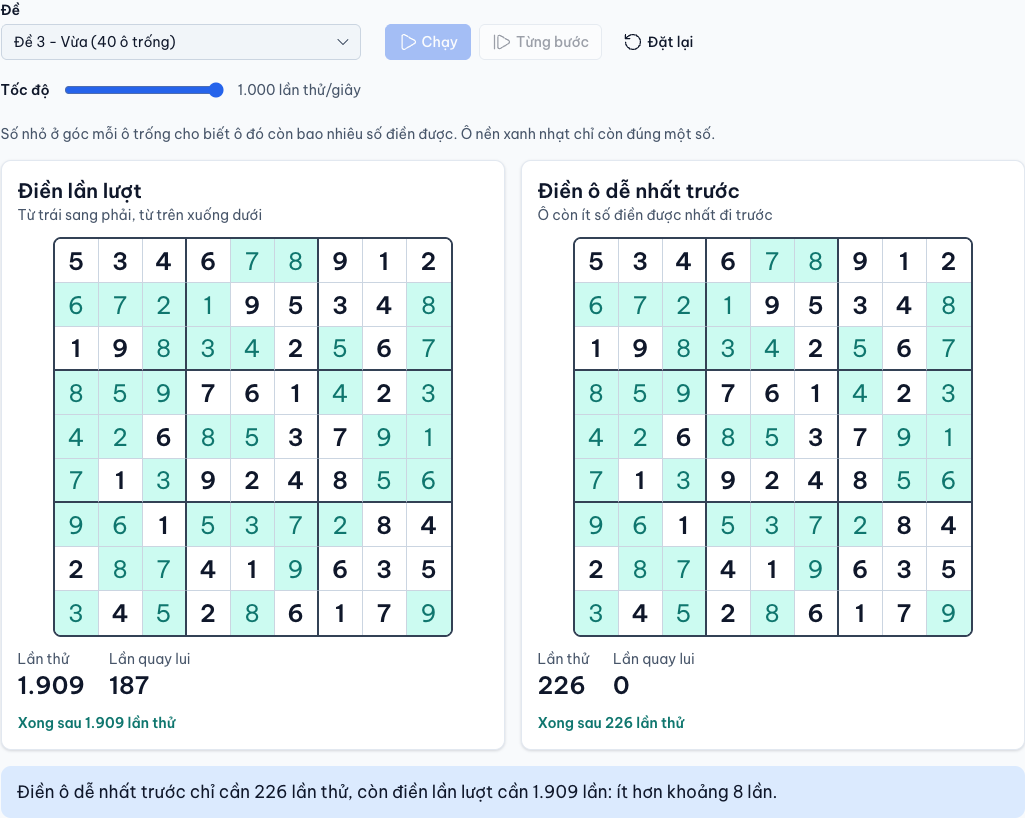
\includegraphics[width=0.92\linewidth]{figures/comparison-race.png}
  \caption{Cuộc đua trên đề ``Vừa'': điền ô dễ nhất trước xong sau 226 lần thử, điền lần lượt cần 1.909 lần}
  \label{fig:race}
\end{figure}

Để có đáp án độc lập, Claude viết thêm một bản Python cho cách điền ô ít khả năng nhất trước. Bản này khớp bản TypeScript trên cả 12 đề.

\section{Trang Mọi lời giải (6/10)}

Mô hình 1 trên slide vốn không dừng ở lời giải đầu: xuất xong một lời giải, nó trả lại trạng thái cũ rồi thử tiếp. Em chọn đặt chế độ ``tìm hết'' ở một trang riêng để trang Giải Sudoku giữ nguyên.

Khi chạy bản Python đếm lời giải, Claude phát hiện đề mẫu ``Vừa'', đề mặc định của trình giải, có 4 lời giải chứ không phải 1. Bộ đếm độc lập trong bộ testcase cũng ra 4. Em sửa lại các chỗ tài liệu ghi sai điều này.

Claude kiểm chéo thêm: chế độ tìm hết đếm lại số lời giải của 251 đề trong bộ testcase. 239 đề tìm hết trong giới hạn 300 nghìn lần thử, và cả 239 đề khớp bộ đếm độc lập. Lỗi tìm ra khi chụp màn hình: ở màn hình rộng 820 px, chữ trong menu sáu mục dồn xuống hai dòng. Claude đo thấy sáu mục vừa một dòng từ 880 px, nên cho menu thu gọn dưới 900 px.

\section{Quy tắc văn phong và viết lại chữ trên website (6/10)}

Em dán ba bộ quy tắc văn phong, bắt đầu bằng:

\begin{promptbox}{6/10}
Nguyên tắc dành cho bạn khi làm việc với câu chữ, hãy lưu vào system\\
• Quy tắc chống văn phong AI (Anti-AI Patterns): Cấm dùng các từ ngữ sáo rỗng, cầu kỳ quá mức (ví dụ: “trong bức tranh toàn cảnh”, “tóm lại là”, “không thể phủ nhận rằng”), ưu tiên câu ngắn, nhịp điệu linh hoạt.\\
• Quy chuẩn mạch lạc (Flow): Hướng dẫn cách chuyển ý tự nhiên giữa các đoạn, đi từ ví dụ thực tế rồi mới rút ra kết luận thay vì áp đặt lý thuyết khô khan
\end{promptbox}

Claude chỉ ra ba chỗ các bộ quy tắc mâu thuẫn nhau hoặc mâu thuẫn với bài làm. Cấu trúc ``câu chuyện trước'' ngược với ``kết luận trước''. Luật ``không đưa code'' đụng tới mã giả cô chấm. Giọng hài hước không hợp với report. Claude đề xuất chia quy tắc theo nơi dùng: website dùng đủ cả bộ, report chỉ dùng luật về câu và bộ lọc từ.

\begin{promptbox}{6/10}
Yeah, về mã giả thì bất khả xâm phạm, tôi đồng ý
\end{promptbox}

\begin{promptbox}{6/10}
Sao bạn không lưu vào như 1 SKILL?
\end{promptbox}

Bộ quy tắc thành một skill của Claude Code, có bước tự kiểm trước khi giao chữ. Em đưa thêm một bài viết mẫu. Claude chỉ ra hai lỗi thuật toán trong bài: ``điền bừa một số'' (thuật toán thử lần lượt từ 1 đến 9, không có gì bừa) và ``thử hết tất cả các trường hợp'' (thuật toán bỏ ngay số trùng, nên đề Inkala chỉ cần 445.778 lần thử thay vì $9^{60}$).

Claude viết lại khoảng 50 câu trên website. Bảng \ref{tab:rewrite} có ba ví dụ.

\begin{table}[H]
  \centering
  \caption{Ba câu trước và sau khi viết lại}
  \label{tab:rewrite}
  \begin{tabularx}{\linewidth}{@{}LL@{}}
    \toprule
    \textbf{Trước} & \textbf{Sau} \\
    \midrule
    Xem thuật toán quay lui giải Sudoku, từng bước một. & Máy giải Sudoku cũng đoán sai. Xem nó lùi lại và sửa. \\
    Ô (4, 7) - thử số 2: bị loại vì 2 đã có ở hàng 4. & Ô (4, 7) - thử số 2: hàng 4 đã có số 2, bỏ. \\
    Nói cách khác, O($9^n$) ở phần trên không chỉ là chuyện lý thuyết. & O($9^n$) ở phần trên không chỉ nằm trên giấy: đề này bắt thuật toán đi gần hết cái cây đó. \\
    \bottomrule
  \end{tabularx}
\end{table}

Lần viết lại này để lọt một lỗi. Ba câu mới có chỗ chờ điền số, nhưng code chưa truyền số vào, nên trang hiện nguyên dấu ngoặc nhọn. Không test nào bắt được. Claude tự phát hiện ngay sau khi commit, sửa, rồi thêm một test mở từng trang và khẳng định không còn chỗ chờ điền nào hiện ra. Lần đầu chính test này vẫn đạt trên bản lỗi, vì nó đọc chữ khi trang còn đang tải. Claude đổi sang chờ trang tải xong, và test báo lỗi đúng ở trang Thuật toán.

\section{Đề minh họa và sự cố máy chậm (8/10 - 10/10)}

Chương 5 cần một đề đủ ngắn để in trọn từng bước, mà vẫn có quay lui. Claude viết script tìm đề theo tiêu chí: 10 đến 16 ô trống, đúng một lời giải, 50 đến 90 lần thử, 1 đến 3 lần quay lui, có đủ ba kiểu bị loại. Script ra 12 đề. Em chọn đề 79 lần thử, 3 lần quay lui, vì cả ba lần quay lui nằm gọn trong 35 lần thử đầu trên hàng 1, và có một lần lùi dây chuyền qua hai ô. Đề này thành đề mẫu số 13 trên website. Một script khác xuất cả 83 bước bằng chính bộ giải của website, nên bảng ở Chương 5 khớp với demo.

Ngày 9/10, \texttt{yarn test} từ 9 giây thành 16 phút, mỗi lần chạy hỏng một test khác nhau vì quá giờ. Claude đo bằng một vòng lặp: cần 1,9 giây CPU mà mất 27 giây, tức máy chỉ cấp khoảng 5 đến 7 phần trăm sức chạy. Máy không bật tiết kiệm pin, cũng không có cảnh báo nhiệt. Claude nới giới hạn thời gian mỗi test lên 30 giây. Ngày 10/10 máy chạy bình thường trở lại, và toàn bộ test đạt: 723 test đơn vị, 292 testcase, 60 test trên Chrome.

\section{Phần việc của em và phần việc của AI}

Bảng \ref{tab:roles} tách phần em làm và phần Claude làm.

\begin{table}[H]
  \centering
  \caption{Phân chia công việc}
  \label{tab:roles}
  \begin{tabularx}{\linewidth}{@{}>{\raggedright\arraybackslash}p{3.4cm}LL@{}}
    \toprule
    \textbf{Việc} & \textbf{Em} & \textbf{Claude} \\
    \midrule
    Chọn đề, phạm vi, công nghệ & Quyết định mọi lựa chọn & Đề xuất phương án, đo đạc để em chọn \\
    Thuật toán & Tự cài đặt quay lui theo mô hình 1 bằng Python từ trước & Chuyển sang TypeScript, giữ đúng cấu trúc; viết thêm biến thể MRV và tìm hết \\
    Giao diện & Duyệt bản thiết kế, thêm yêu cầu Sáng và Tối, góp ý từng màn hình & Claude Code soạn prompt; Claude Design vẽ; Claude Code code theo bản vẽ \\
    Code website, script, test & Duyệt kết quả qua ảnh chụp và chạy thử & Viết toàn bộ code, test, script đo đạc \\
    Chữ trên website & Đặt quy tắc văn phong, sửa các câu chưa tự nhiên & Viết nháp theo quy tắc \\
    Kiểm chứng & Yêu cầu soát lại khi thấy lạ (trang So sánh, thời gian chạy) & Đề xuất và chạy các cách soát: bản Python độc lập, cố tình làm sai, chụp màn hình \\
    Report & Đọc, sửa và chịu trách nhiệm nội dung & Viết bản nháp từ nhật ký và transcript \\
    \bottomrule
  \end{tabularx}
\end{table}

Các cách kiểm chứng em dựa vào xuyên suốt dự án:

\begin{itemize}
  \item \textbf{Đáp án độc lập.} Mọi con số trên website và trong report đều so với bản Python viết riêng: bản tham chiếu mô hình 1, bản điền ô ít khả năng nhất trước, bản tìm hết, và bộ đếm lời giải dùng cách khác hẳn.
  \item \textbf{Cố tình làm sai.} Mỗi khi test đạt hết ngay lần đầu, Claude đưa lỗi vào thuật toán để xem test có bắt được không. Hai lần cách này lộ ra lỗ hổng thật.
  \item \textbf{Chụp màn hình trên Chrome thật} ở nhiều cỡ màn hình, sáng và tối, trên điện thoại.
  \item \textbf{Số đo thật thay cho phỏng đoán}, từ số bước giữ trong lịch sử tới chiều rộng menu.
\end{itemize}

\chapter{Thiết kế thực nghiệm}

\section{Cách tạo bộ testcase}

\section{Các nhóm testcase}

\section{Cách bảo đảm độ phủ}

\section{Đáp án lấy từ đâu}

\chapter{Đánh giá}

Lần chạy đầy đủ ngày 12/10/2026, kể cả hai đề chậm, cho cả 294 đề của bộ testcase đạt. Ngày 13/10/2026, 772 test đơn vị và 76 test trên Chrome cũng đạt. Các số đo trong chương chạy trên máy Apple M2 Pro, RAM 16 GB, macOS 26.7, Node 24.13 và Chrome 154. Số đo thời gian phụ thuộc máy, còn số lần thử thì không.

\section{Kết quả trên bộ testcase}

Lệnh \texttt{yarn testcases --include-slow} chạy cả 294 đề, kể cả 2 đề chậm, và cả 294 đề đạt (Bảng \ref{tab:testcase-groups}). Mỗi đề phải khớp đáp án ở bốn chỗ: loại kết quả, nội dung đầu ra, ba bộ đếm, và ba số lần bị loại theo hàng, cột, khối. Cả bộ đi qua đủ 20 nhánh xử lý.

Kết quả từng đề lưu trong \texttt{testcases/results/results.csv}. Lệnh \texttt{yarn testcases} không kèm 2 đề chậm chạy lại 292 đề còn lại trong khoảng 9 giây.

\section{Thời gian thực hiện}

\begin{itemize}
  \item \textbf{Đề nhỏ và đề thông thường} chạy dưới 30 ms mỗi đề trên bộ giải của website.
  \item \textbf{Đề chậm nhất trong nhóm chạy mặc định} là Easter Monster: 2.357.880 lần thử, 3,37 giây.
  \item \textbf{Hai đề chậm:} đề chống quay lui mất 13 phút 57 giây, đề 17 số mất 4 phút 45 giây.
\end{itemize}

Phần lớn thời gian đó tốn vào việc minh họa từng bước. Bộ giải của website là một generator, và mỗi sự kiện phải đi qua từng tầng đệ quy mới tới giao diện (Chương 4). Trên đề Arto Inkala, bản generator mất 596 ms, bản đệ quy thường của trang So sánh mất 4,42 ms, chậm hơn khoảng 135 lần. Phép đo này chạy riêng với bảng so sánh ở mục sau, và cùng bản đệ quy đó trong bảng mất 5,17 ms, lệch khoảng 15 phần trăm, nên các tỉ lệ chỉ nên đọc là gần đúng. Trên ba đề mẫu khác, tỉ lệ này từ 63 đến 104 lần (\texttt{report/data/generator-overhead.csv}).

Trên Node, bộ giải của website chạy khoảng 744 nghìn lần thử mỗi giây. Nút Giải ngay trên Chrome giải đề Inkala trong khoảng 0,6 giây, tức khoảng 770 nghìn lần thử mỗi giây. Người xem bấm Dừng được bất cứ lúc nào, trang không treo.

\section{So sánh các cách giải}

Trang So sánh đo 6 cách: 2 thứ tự chọn ô nhân với 3 cách kiểm tra. Sáu đề đo là sáu đề mẫu cần nhiều lần thử nhất, không tính lưới trống vì lưới trống không phải một đề thật. Bảng \ref{tab:comparison-tries} và Bảng \ref{tab:comparison-times} là kết quả chạy bằng script \texttt{report/tools/measureComparison.ts} ngày 12/10. Script dùng đúng hàm đo của trang So sánh: mỗi cách chạy lặp lại tới khi đủ 0,3 giây hoặc đủ 10.000 lần, rồi lấy trung bình.

\begin{table}[H]
  \centering
  \caption{Số lần thử theo thứ tự chọn ô (ba cách kiểm tra cho cùng một số)}
  \label{tab:comparison-tries}
  \small
  \begin{tabular}{@{}lrrrr@{}}
\toprule
\textbf{Đề} & \textbf{Ô trống} & \textbf{Điền lần lượt} & \textbf{Ô dễ nhất trước} & \textbf{Giảm} \\
\midrule
Vừa & 40 & 1.909 & 226 & 8 lần \\
Wikipedia & 51 & 37.652 & 239 & 158 lần \\
Arto Inkala & 60 & 445.778 & 90.665 & 5 lần \\
AI Escargot & 58 & 80.491 & 1.723 & 47 lần \\
Easter Monster & 60 & 2.357.880 & 42.081 & 56 lần \\
Chống quay lui & 64 & 622.577.597 & 407.156 & 1.529 lần \\
\bottomrule
\end{tabular}

\end{table}

\begin{table}[H]
  \centering
  \caption{Thời gian mỗi lần giải, tính bằng mili giây. Lưới: quét lại lưới; Sổ: ba mảng đánh dấu; Công tắc: bitmask}
  \label{tab:comparison-times}
  \small
  \begin{tabular}{@{}lrrrrrr@{}}
\toprule
 & \multicolumn{3}{c}{\textbf{Điền lần lượt}} & \multicolumn{3}{c}{\textbf{Ô dễ nhất trước}} \\
\cmidrule(lr){2-4}\cmidrule(l){5-7}
\textbf{Đề} & Lưới & Sổ & Công tắc & Lưới & Sổ & Công tắc \\
\midrule
Vừa & 0,034 & 0,021 & 0,021 & 0,144 & 0,046 & 0,045 \\
Wikipedia & 0,750 & 0,396 & 0,381 & 0,275 & 0,078 & 0,070 \\
Arto Inkala & 9,55 & 5,17 & 4,67 & 81,9 & 23,5 & 20,5 \\
AI Escargot & 1,76 & 0,961 & 0,848 & 1,45 & 0,434 & 0,373 \\
Easter Monster & 53,3 & 29,3 & 24,6 & 33,9 & 10,6 & 8,74 \\
Chống quay lui & 17.632 & 8.588 & 8.892 & 767 & 170 & 167 \\
\bottomrule
\end{tabular}

\end{table}

Cấu trúc dữ liệu chỉ đổi hằng số. Ba cách kiểm tra cho đúng cùng số lần thử trên mọi đề, đúng như phân tích ở Chương 4: cách kiểm tra chỉ đổi \(c_2\) trong \(T(n) = 9\,T(n-1) + c_2\). Quét lưới chậm khoảng gấp đôi ba mảng đánh dấu, ví dụ 9,55 ms so với 5,17 ms trên đề Inkala. Bitmask nhanh hơn ba mảng đánh dấu khoảng 4 đến 16 phần trăm ở bốn đề, bằng nhau ở đề Vừa, và chậm hơn ở đề chống quay lui: 8.892 ms so với 8.588 ms.

Thứ tự chọn ô thì đổi cả cây tìm kiếm. Cách chọn ô ít khả năng nhất trước (MRV, trên website gọi là ``Điền ô dễ nhất trước'') cần ít lần thử hơn ở cả sáu đề. Mức giảm ít nhất ở đề Inkala, khoảng 5 lần (445.778 xuống 90.665), nhiều nhất ở đề chống quay lui, khoảng 1.529 lần (622.577.597 xuống 407.156).

Ít lần thử hơn chưa chắc nhanh hơn. Trước mỗi bước, MRV phải đếm lại khả năng của mọi ô trống còn lại. Ở đề Vừa và đề Inkala, số lần thử giảm chưa đủ bù phần đếm đó, nên tổng thời gian dài hơn: đề Inkala 23,5 ms so với 5,17 ms. Ở bốn đề còn lại, số lần thử giảm từ khoảng 47 lần trở lên và cách này nhanh hơn rõ: đề chống quay lui từ 8,6 giây xuống 0,17 giây, đề Easter Monster từ 29,3 ms xuống 10,6 ms.

\section{Kiểm thử tự động}

\begin{itemize}
  \item \textbf{772 test đơn vị} (Vitest):
  \begin{itemize}
    \item bộ giải khớp bản Python đến từng con số trên các đề mẫu;
    \item trạng thái lưới khớp các khung của bản thiết kế;
    \item ba cách kiểm tra và MRV khớp bản Python riêng của chúng;
    \item chế độ tìm hết khớp số lời giải;
    \item lịch sử lùi từ 1 đến 300 sự kiện vẫn ra đúng trạng thái;
    \item câu thông báo đúng từng ký tự;
    \item toàn bộ 292 đề nhanh của bộ testcase;
    \item bộ giải theo kích thước lưới khớp bản Python trên 11 đề và phát ra đúng chuỗi sự kiện của bộ giải \(9 \times 9\) trên 8 đề.
  \end{itemize}
  \item \textbf{76 test trên Chrome thật} (Playwright): mọi trạng thái trong bản thiết kế, các nút Từng bước, Tự động, Giải ngay, Dừng, lịch sử, cuộc đua và phép đo ở trang So sánh, trang Mọi lời giải, bố cục ở nhiều cỡ màn hình từ 320 đến 2560 px, và không trang nào hiện chỗ chờ điền chưa thay số.
  \item \textbf{Soát code:} TypeScript ở chế độ nghiêm ngặt, oxlint, không còn chữ tiếng Việt nào trong code ngoài file ngôn ngữ.
\end{itemize}

Claude kiểm lại chính bộ test bằng các lỗi cố ý (Bảng \ref{tab:mutations}). Lần đầu, bộ test để lọt hai trong bốn lỗi. Claude vá cả hai lỗ hổng, và bộ test sau đó bắt được cả bốn.

\section{Tính trực quan của giao diện}

Phần minh họa cho người xem thấy cùng lúc bốn thứ: lưới với màu riêng cho từng trạng thái ô, dòng mã giả đang chạy kèm nhãn đúng hoặc sai, vectơ \(S\), và một câu giải thích bằng lời, ví dụ ``Ô (4, 7) - thử số 2: hàng 4 đã có số 2, bỏ''. Các chức năng hỗ trợ người học:

\begin{itemize}
  \item Từng bước, lùi một bước, tự động với tốc độ từ 1 đến 1.000 lần thử mỗi giây, tới lần quay lui kế tiếp, giải ngay.
  \item Chạy tự động thì dừng ở lần quay lui đầu tiên và hỏi người xem đoán bước tiếp theo.
  \item Bảng lịch sử 100 bước gần nhất, bấm vào một dòng để xem lại đúng trạng thái lúc đó.
  \item Cuộc đua hai lưới ở trang So sánh, mỗi ô trống hiện số khả năng còn lại.
  \item Bộ sưu tập lời giải ở trang Mọi lời giải, tô các ô khác lời giải đầu tiên.
  \item Trang Kích thước lưới chạy cùng mã giả trên lưới \(4 \times 4\), \(9 \times 9\) và \(16 \times 16\), kèm bảng số lần thử của 11 đề mẫu.
\end{itemize}

Về khả năng tiếp cận, các cặp màu chữ và nền đạt độ tương phản WCAG AA. Mỗi trạng thái ô có thêm dấu hiệu ngoài màu, ví dụ gạch ngang cho số bị loại và viền nét đứt cho ô vừa trả lại. Lưới đi được bằng phím mũi tên. Trang có chế độ tối, có bố cục riêng cho điện thoại, và hoạt ảnh ở trang chủ đứng yên khi máy bật giảm chuyển động.

Em chưa kiểm thử với người dùng thật. Các góp ý về giao diện và câu chữ đến từ việc em tự dùng thử, cộng với các phiên Claude và agent đóng vai người dùng phổ thông, sinh viên và biên tập viên (Chương 6). Đây là hạn chế lớn nhất của phần đánh giá giao diện.

\section{Hạn chế và hướng phát triển}

\subsection*{Hạn chế}

\begin{itemize}
  \item Để minh họa từng bước, bộ giải trên website chậm hơn bản đệ quy thường từ 63 đến 135 lần tùy đề, 135 lần ở đề Inkala. Theo tốc độ đo trên Chrome, đề chống quay lui cần khoảng 14 phút khi bấm Giải ngay.
  \item Chưa có người dùng thật thử.
  \item MRV mới có ở trang So sánh, chưa chạy từng bước được ở trang Giải Sudoku.
  \item Trang Kích thước lưới chỉ có 11 đề mẫu cố định, chưa cho dán hay gõ đề riêng. Các đề \(16 \times 16\) sinh ngẫu nhiên nên một số có nhiều lời giải.
  \item Đề ngẫu nhiên trong bộ testcase nghiêng về phía dễ, vì script bỏ các đề cần hơn 1 triệu lần thử.
  \item Đáp án của bộ testcase và bộ giải của website cùng do Claude viết (Chương 7).
  \item Lịch sử chỉ giữ 100 bước gần nhất. Muốn xem lại bước cũ hơn thì phải chạy lại từ đầu.
  \item Website chỉ có tiếng Việt, dù toàn bộ chữ đã tách sẵn ra một file để dịch.
\end{itemize}

\subsection*{Hướng phát triển}

\begin{itemize}
  \item Cho trang Giải Sudoku chọn MRV và chạy từng bước.
  \item Chạy Giải ngay bằng bản đệ quy thường trong một luồng riêng của trình duyệt (Web Worker), chỉ dùng generator khi cần xem từng bước.
  \item Cho trang Kích thước lưới nhận đề do người dùng dán, và thêm các cỡ khác như \(25 \times 25\).
  \item Dùng lại phần minh họa cho các bài quay lui khác trong slide: 8 quân hậu, tổng tập con, tô màu đồ thị.
  \item Thử với một nhóm người học thật, ghi lại chỗ họ không hiểu.
  \item Thêm bản tiếng Anh.
\end{itemize}


\end{document}
